%----------
%   IMPORTANTE
%----------

% Si nunca has utilizado LaTeX es conveniente que aprendas una serie de conceptos básicos antes de utilizar esta plantilla. Te aconsejamos que leas previamente algún tutorial (puedes encontar muchos en Internet).

% Esta plantilla está basada en las recomendaciones de la guía "Trabajo fin de Máster: Escribir el TFM", que encontrarás en http://uc3m.libguides.com/TFM/escribir
% contiene recomendaciones de la Biblioteca basadas principalmente en estilos APA e IEEE, pero debes seguir siempre las orientaciones de tu Tutor de TFM y la normativa de TFM para tu titulación.

% Encontrarás un ejemplo de TFM realizado con esta misma plantilla en la carpeta "_ejemplo_TFM_2019". Consúltalo porque contiene ejemplos útiles para incorporar tablas, figuras, listados de código, bibliografía, etc.



%----------
%	CONFIGURACIÓN DEL DOCUMENTO
%----------

% Definimos las características del documento y añadimos una serie de paquetes (\usepackage{package}) que agregan funcionalidades a LaTeX.

\documentclass[12pt]{report} %fuente a 12pt

%------------------------------------------------------------------------------------

\hyphenation{pro-por-cio-na-do in-fra-es-truc-tu-ra he-rra-mien-tas im-ple-men-ta-ciones Win-dows si-guien-tes prin-ci-pa-les op-ti-mi-za-da de-sa-rro-llar com-par-ti-das In-te-rac-ti-ve lle-van-do de-no-mi-na-da Win-Log-on ins-tan-ciar se-gu-ri-dad al-go-rit-mos al-ma-ce-nan Prin-ci-pal com-pro-bar siem-pre su-fi-cien-tes co-rres-pon-dien-tes al-ma-ce-nan  sis-te-mas ac-tu-al-men-te con-fi-den-cia-li-dad pos-te-rior-men-te coin-ci-de ac-tu-ar co-rres-pon-dien-te acce-der sir-ve per-te-ne-cien-tes per-te-ne-cien-tes de-sa-rro-lla-do con-fi-gu-ra le-van-tan po-de-mos e-je-cu-ta-mos in-ter-cep-ta-da ob-te-ner-las pro-por-cio-na-da}

% \hyphenation{ciber-delincuentes pro-por-cionadas com-pro-meter ges-tio-nar la-bo-ra-torio net-working pro-por-cio-na-do cen-tra-li-za-da im-ple-men-ta-do he-rra-mien-tas in-fra-es-truc-tu-ra Di-rec-to-ry im-ple-men-ta-cio-nes auten-ti-ca-cion u-ti-li-za-dos} 
\PassOptionsToPackage{hyphens}{url}
\usepackage{float}
\UseRawInputEncoding

\usepackage{cite}


\usepackage{color}
\definecolor{gray97}{gray}{.97}
\definecolor{gray75}{gray}{.75}
\definecolor{gray45}{gray}{.45}

\usepackage{listings}
\lstset{ frame=Ltb,
framerule=0pt,
aboveskip=0.5cm,
framextopmargin=3pt,
framexbottommargin=3pt,
framexleftmargin=0.4cm,
framesep=0pt,
rulesep=.4pt,
backgroundcolor=\color{gray97},
rulesepcolor=\color{black},
%
stringstyle=\ttfamily,
showstringspaces = false,
basicstyle=\small\ttfamily,
commentstyle=\color{gray45},
keywordstyle=\bfseries,
%
numbers=left,
numbersep=15pt,
numberstyle=\tiny,
numberfirstline = false,
breaklines=true,
}

% minimizar fragmentado de listados
\lstnewenvironment{listing}[1][]
{\lstset{#1}\pagebreak[0]}{\pagebreak[0]}

\lstdefinestyle{consola}
{basicstyle=\scriptsize\bf\ttfamily,
backgroundcolor=\color{gray75},
}

\lstdefinestyle{C}
{language=C,
}

%------------------------------------------------------------------------------------



% MÁRGENES: 2,5 cm sup. e inf.; 3 cm izdo. y dcho.
\usepackage[
a4paper,
vmargin=2.5cm,
hmargin=3cm
]{geometry}

% INTERLINEADO: Estrecho (6 ptos./interlineado 1,15) o Moderado (6 ptos./interlineado 1,5)
\renewcommand{\baselinestretch}{1.15}
\parskip=6pt

% DEFINICIÓN DE COLORES para portada y listados de código
\usepackage[table]{xcolor}
\definecolor{azulUC3M}{RGB}{0,0,102}
\definecolor{gray97}{gray}{.97}
\definecolor{gray75}{gray}{.75}
\definecolor{gray45}{gray}{.45}

% Soporte para GENERAR PDF/A --es importante de cara a su inclusión en e-Archivo porque es el formato óptimo de preservación y a la generación de metadatos, tal y como se describe en http://uc3m.libguides.com/ld.php?content_id=31389625. En la carpeta incluímos el archivo plantilla_tfg_2017.xmpdata en el que puedes incluir los metadatos que se incorporarán al archivo PDF cuando lo compiles. Ese archivo debe llamarse igual que tu archivo .tex. Puedes ver un ejemplo en esta misma carpeta.
\usepackage[a-1b]{pdfx}

% ENLACES
\usepackage{hyperref}
\hypersetup{colorlinks=true,
	linkcolor=black, % enlaces a partes del documento (p.e. índice) en color negro
	urlcolor=blue} % enlaces a recursos fuera del documento en azul

% EXPRESIONES MATEMATICAS
\usepackage{amsmath,amssymb,amsfonts,amsthm}

\usepackage{txfonts} 
\usepackage[T1]{fontenc}
\usepackage[utf8]{inputenc}

\usepackage[spanish, es-tabla]{babel} 
\usepackage[babel, spanish=spanish]{csquotes}
\AtBeginEnvironment{quote}{\small}

% diseño de PIE DE PÁGINA
\usepackage{fancyhdr}
\pagestyle{fancy}
\fancyhf{}
\renewcommand{\headrulewidth}{0pt}
\rfoot{\thepage}
\fancypagestyle{plain}{\pagestyle{fancy}}

% DISEÑO DE LOS TÍTULOS de las partes del trabajo (capítulos y epígrafes o subcapítulos)
\usepackage{titlesec}
\usepackage{titletoc}

\titleformat{\chapter}[block]
{\large\bfseries} %\filcenter}
{\thechapter.}
{5pt}
{}
{}
\titlespacing{\chapter}{0pt}{0pt}{*3}
\titlecontents{chapter}
[0pt]                                               
{}
{\contentsmargin{0pt}\thecontentslabel.\enspace}
{\contentsmargin{0pt}}                        
{\titlerule*[.7pc]{.}\contentspage}                 

\titleformat{\section}
{\bfseries}
{\thesection.}
{5pt}
{}
\titlecontents{section}
[5pt]                                               
{}
{\contentsmargin{0pt}\thecontentslabel.\enspace}
{\contentsmargin{0pt}}
{\titlerule*[.7pc]{.}\contentspage}

\titleformat{\subsection}
{\normalsize\bfseries}
{\thesubsection.}
{5pt}
{}
\titlecontents{subsection}
[10pt]                                               
{}
{\contentsmargin{0pt}                          
	\thecontentslabel.\enspace}
{\contentsmargin{0pt}}                        
{\titlerule*[.7pc]{.}\contentspage}  


% DISEÑO DE TABLAS. Puedes elegir entre el estilo para ingeniería o para ciencias sociales y humanidades. Por defecto, está activado el estilo de ingeniería. Si deseas utilizar el otro, comenta las líneas del diseño de ingeniería y descomenta las del diseño de ciencias sociales y humanidades
\usepackage{multirow} % permite combinar celdas 
\usepackage{caption} % para personalizar el título de tablas y figuras
% \usepackage{floatrow} % utilizamos este paquete y sus macros \ttabbox y \ffigbox para alinear los nombres de tablas y figuras de acuerdo con el estilo definido. Para su uso ver archivo de ejemplo 
\usepackage{array} % con este paquete podemos definir en la siguiente línea un nuevo tipo de columna para tablas: ancho personalizado y contenido centrado
\newcolumntype{P}[1]{>{\centering\arraybackslash}p{#1}}
\DeclareCaptionFormat{upper}{#1#2\uppercase{#3}\par}

% Diseño de tabla para ingeniería
\captionsetup[table]{
	format=upper,
	name=TABLA,
	justification=centering,
	labelsep=period,
	width=.75\linewidth,
	labelfont=small,
	font=small,
}

%Diseño de tabla para ciencias sociales y humanidades
%\captionsetup[table]{
%	justification=raggedright,
%	labelsep=period,
%	labelfont=small,
%	singlelinecheck=false,
%	font={small,bf}
%}


% DISEÑO DE FIGURAS. Puedes elegir entre el estilo para ingeniería o para ciencias sociales y humanidades. Por defecto, está activado el estilo de ingeniería. Si deseas utilizar el otro, comenta las líneas del diseño de ingeniería y descomenta las del diseño de ciencias sociales y humanidades
\usepackage{graphicx}
\graphicspath{{imagenes/}} %ruta a la carpeta de imágenes

% Diseño de figuras para ingeniería
\captionsetup[figure]{
	format=hang,
	name=Fig.,
	singlelinecheck=off,
	labelsep=period,
	labelfont=small,
	font=small		
}

% Diseño de figuras para ciencias sociales y humanidades
%\captionsetup[figure]{
%	format=hang,
%	name=Figura,
%	singlelinecheck=off,
%	labelsep=period,
%	labelfont=small,
%	font=small		
%}


% NOTAS A PIE DE PÁGINA
\usepackage{chngcntr} %para numeración contínua de las notas al pie
\counterwithout{footnote}{chapter}

% LISTADOS DE CÓDIGO
% soporte y estilo para listados de código. Más información en https://es.wikibooks.org/wiki/Manual_de_LaTeX/Listados_de_código/Listados_con_listings
\usepackage{listings}

% definimos un estilo de listings
\lstdefinestyle{estilo}{ frame=Ltb,
	framerule=0pt,
	aboveskip=0.5cm,
	framextopmargin=3pt,
	framexbottommargin=3pt,
	framexleftmargin=0.4cm,
	framesep=0pt,
	rulesep=.4pt,
	backgroundcolor=\color{gray97},
	rulesepcolor=\color{black},
	%
	basicstyle=\ttfamily\footnotesize,
	keywordstyle=\bfseries,
	stringstyle=\ttfamily,
	showstringspaces = false,
	commentstyle=\color{gray45},     
	%
	numbers=left,
	numbersep=15pt,
	numberstyle=\tiny,
	numberfirstline = false,
	breaklines=true,
	xleftmargin=\parindent
}

\captionsetup[lstlisting]{font=small, labelsep=period}
% fijamos el estilo a utilizar 
\lstset{style=estilo}
\renewcommand{\lstlistingname}{\uppercase{Código}}


%BIBLIOGRAFÍA - PUEDES ELEGIR ENTRE ESTILO IEEE O APA. POR DEFECTO ESTÁ CONFIGURADO IEEE. SI DESEAS USAR APA, COMENTA LAS LÍNEA DE IEEE Y DESCOMENTA LAS DE APA. Si haces cambios en la configuración de la bibliografía y no obtienes los resultados esperados, es recomendable limpiar los archivos auxiliares y volver a compilar en este orden: COMPILAR-BIBLIOGRAFIA-COMPILAR

% Tienes más información sobre cómo generar bibliografía y CONFIGURAR TU EDITOR DE TEXTO para compilar con biber en http://tex.stackexchange.com/questions/154751/biblatex-with-biber-configuring-my-editor-to-avoid-undefined-citations , https://www.overleaf.com/learn/latex/Bibliography_management_in_LaTeX y en http://www.ctan.org/tex-archive/macros/latex/exptl/biblatex-contrib
% También te recomendamos consultar la guía temática de la Biblioteca sobre citas bibliográficas: http://uc3m.libguides.com/guias_tematicas/citas_bibliograficas/inicio

% CONFIGURACIÓN PARA LA BIBLIOGRAFÍA IEEE
% \usepackage[backend=biber, style=ieee, isbn=false,sortcites, maxbibnames=5, minbibnames=1]{biblatex} % Configuración para el estilo de citas de IEEE, recomendado para el área de ingeniería. "maxbibnames" indica que a partir de 5 autores trunque la lista en el primero (minbibnames) y añada "et al." tal y como se utiliza en el estilo IEEE.

%CONFIGURACIÓN PARA LA BIBLIOGRAFÍA APA
%\usepackage[style=apa, backend=biber, natbib=true, hyperref=true, uniquelist=false, sortcites]{biblatex}
%\DeclareLanguageMapping{spanish}{spanish-apa}

% Añadimos las siguientes indicaciones para mejorar la adaptación de los estilos en español
% \DefineBibliographyStrings{spanish}{%
% 	andothers = {et\addabbrvspace al\adddot}
% }
% \DefineBibliographyStrings{spanish}{
% 	url = {\adddot\space[En línea]\adddot\space Disponible en:}
% }
% \DefineBibliographyStrings{spanish}{
% 	urlseen = {Acceso:}
% }
% \DefineBibliographyStrings{spanish}{
% 	pages = {pp\adddot},
% 	page = {p.\adddot}
% }

% \addbibresource{Bibliografia/Bibliografia.bib} % llama al archivo bibliografia.bib en el que debería estar la bibliografía utilizada


%-------------
%	DOCUMENTO
%-------------

\begin{document}
\pagenumbering{roman} % Se utilizan cifras romanas en la numeración de las páginas previas al cuerpo del trabajo
	

%----------
%	PORTADA
%----------	

\thispagestyle{empty}


%----------
%	PORTADA
%----------	
\begin{titlepage}
	\begin{sffamily}
	\color{azulUC3M}
	\begin{center}
		\begin{figure}[H] %incluimos el logotipo de la Universidad
			\makebox[\textwidth][c]{
\includegraphics[width=16cm]{Portada_Logo.png}}
		\end{figure}
		\vspace{1cm}
		\begin{Large}
			Máster Universitario en Ciberseguridad\\			
			2018-2019\\
			\vspace{1cm}		
			\textsl{Trabajo Fin de Máster}
			\bigskip
			
		\end{Large}
		 	% {\Huge ``CIBEREJERCICIOS PARA EVALUAR ACTIVE DIRECTORY EN SUS DISTINTAS VERSIONES. ''}\\
		 	{\Huge ``Ciberejercicios para evaluar \\
		 	Active Directory en sus distinas versiones. ''}\\
		 	\vspace*{0.5cm}
	 		\rule{10.5cm}{0.1mm}\\
			\vspace*{0.9cm}
			{\LARGE Borja Lorenzo Fernádez}\\ 
			\vspace*{1cm}
		\begin{Large}
			Tutor\\
			Andrés Marín López\\
		\end{Large}
	\end{center}
	
	\vfill
	\color{black}
	\begin{footnotesize}
	\noindent\fbox{
	\begin{minipage}{\textwidth}
		\textbf{DETECCIÓN DEL PLAGIO}\\
		La Universidad utiliza el programa \textbf{Turnitin Feedback Studio} para comparar la originalidad del trabajo entregado por cada estudiante con millones de recursos electrónicos y detecta aquellas partes del texto copiadas y pegadas. Copiar o plagiar en un TFM es considerado una \textbf{\underline{Falta Grave}}, y puede conllevar la expulsión definitiva de la Universidad.
	\end{minipage}	
	}
	% \vspace*{.5cm}\\	
	% \noindent
\includegraphics[width=4.2cm]{imagenes/creativecommons.png}\\
	% \emph{[Incluir en el caso del interés en su publicación en el archivo abierto]}\\
	% Esta obra se encuentra sujeta a la licencia Creative Commons \textbf{Reconocimiento - No Comercial - Sin Obra Derivada}

	\end{footnotesize}
	\end{sffamily}
\end{titlepage}

\newpage %página en blanco o de cortesía
\thispagestyle{empty}
\mbox{}

%----------
%	Agracedimientos
%----------	
\chapter*{Agradecimientos}
%----------
%	Agracedimientos
%----------	

\setcounter{page}{3}
	
	% ESCRIBIR LA DEDICATORIA AQUÍ	


En primer lugar, me gustaría dedicar este trabajo a mis abuelos ya que sin ellos no habría podido llegar a donde he llegado. \\

Agradecer especialmente a mi familia, padres y hermanos por ayudarme y aguantarme incluso en los peores momentos. \\

Quiero agradecer a María, por la dedicación, el esfuerzo y la paciencia que ha tenido conmigo y por habeme enseñado tanto y haberme facilitado las cosas para llegar hasta aquí. \\

Por último, agradecer a todos los que me han ayudado con el desarrollo de este proyecto desinteresadamente, especialemente a Atl4s, Arcocapaz, Cynops y Mamatb.
\vfill
\newpage %página en blanco o de cortesía
\thispagestyle{empty}
\mbox{}


%----------
%	RESUMEN Y PALABRAS CLAVE
%----------	
\chapter*{Resumen}
%----------
%	RESUMEN Y PALABRAS CLAVE
%----------	

\setcounter{page}{5}
	
Active Directory (AD) es una base de datos distribuida que permite a los administradores gestionar de manera eficiente la información de la empresa y los límites de la misma. En la actualidad, Active Directory es considerado una de las partes fundamentales para el correcto funcionamiento de cualquier empresa. La información gestionada por Active Directory, engloba usuarios, clientes, proveedores, dispositivos (ordenadores, servidores, impresoras...), servicios y aplicaciones así como la interacción entre ellos. Por lo tanto, supone uno de los principales objetivos para atacantes y ciberdelincuentes así como una gran problema de seguridad para una organización si el sistema de gestión principal se ve comprometido. En los últimos años se ha producido un gran aumento de ataques contra Active Directory cuyo objetivo es hacerse con el control de la empresa y comprometer la seguridad de la información, esto es debido a que se han perfeccionado los principales ataques así como la implementación de nuevas herramientas que facilitan todo tipo de ataques. \\

Con el fin de contribuir al desarrollo y mejora de la seguridad de Active Directory y por ende, de las empresas y particulares que hacen uso de ello, el trabajo realizado se centra en el estudio de los principales componentes que engloban la seguridad y gestión del sistema de directorio Active Directory a través de la creación de un laboratorio, de manera local, y el análisis y revisión de los principales ataques y amenazas usadas en la actualidad para vulnerar dicho sistema de gestión. Para ello, se implementa una topología que simula una empresa ficticia e implementa la última versión de Windows Server 2019.\\ 

\textit{\textbf{Palabras Clave:}}

Microsoft Active Directory, Domain Controller, Kerberos, Ciberseguridad, Windows Server, Pentesting, Red Team
	
		
\vfill
\newpage %página en blanco o de cortesía
\thispagestyle{empty}
\mbox{}



%-------------------------------------------------------------------------------
%	ÍNDICES
%-------------------------------------------------------------------------------

%--
%Índice general
%-
\tableofcontents
\thispagestyle{fancy}

\newpage %página en blanco o de cortesía
\thispagestyle{empty}
\mbox{}

%--
%Índice de figuras. Si no se incluyen, comenta las líneas siguientes
%-
\listoffigures
\thispagestyle{fancy}

\newpage %página en blanco o de cortesía
\thispagestyle{empty}
\mbox{}

%--
%Índice de tablas. Si no se incluyen, comenta las líneas siguientes
%-
\listoftables
\thispagestyle{fancy}

\newpage %página en blanco o de cortesía
\thispagestyle{empty}
\mbox{}


%-------------------------------------------------------------------------------
%-------------------------------------------------------------------------------

%----------
%	TRABAJO
%----------	
\clearpage
\pagenumbering{arabic} % numeración con múmeros arábigos para el resto de la publicación	


\chapter{Introducción}
En los últimos años, empresas y organizaciones se han visto en la necesidad de gestionar de una manera eficiente y centralizada la información y recursos en red que disponen, activo fundamental para el correcto funcionamiento del negocio. El aumento masivo de dicha información además de la necesidad de crear, distribuir y manipular tal cantidad de datos, ya sea a través de servicios de bases de datos como puede ser servicios MySQL, la obtención de servidores y dispositivos para su almacenamiento, la creación de  aplicaciones web y servicios que permitan su distribución o la gestión de los usuarios que puedan manipularla o consultarla supone una gran cantidad de agentes que intervienen en el funcionamiento que es necesario controlar y regular. Microsoft Active Directory supone una solución a esa problemática a través de un servicio de directorio como base de datos distribuida que permite la gestión, administración y localización de todos los recursos en red ~\cite{Capitulo1:Microsoft}.\\

Dentro del panorama actual, los servicios de Microsoft Active Directory se ha convertido en uno de los pilares que sostienen la organización de los recursos en red de la mayoría de las empresas vigentes así como uno de los principales objetivos para atacantes  debido a dicha importancia. Esto se puede comprobar en el principal interés que tienen los principales grupos de ciberdelincuentes como APT28, Cobalt Strike...  por esta infraestructura o los ataques de ransomware WannaCry, NotPetya, MBR-ONI, etc, que ponen a Active Directory en el punto de mira y centro de sus ataques \cite{Capitulo1:Ransomware}. En los últimos años, se ha visto un aumento considerable de vulnerabilidades críticas que afectan a la seguridad y que detectan y hacen considerablemente más sencillo su explotación. \\

Por todo ello y con el fin de abordar esta problemática, el trabajo realizado se ha centrado en la revisión, análisis y prueba en profundidad de las principales amenazas que suponen un problema de seguridad para Active Directory en sus diferentes versiones, técnicas como Pass-The-Hass, NTLM Relay, Kerberoast, etc que serán detalladas en los capítulos posteriores. Además, también se proporciona las directrices para la creación de un laboratorio local que permite la prueba de los ataques detallados así como la posibilidad de probar nuevas técnicas y ataques sin poner en riesgo la seguriidad de ningún entorno real u organización.\\


\section{Estado del Arte}

Para el desarrollo del trabajo, se ha considerado las siguientes versiones proporcionadas por Microsoft para la instalación de los dominios que van a formar partes del Active Directory y van a ejecutar los Domain Controllers:\\

\begin{itemize}
\item \textbf{Windows Server 2019}
\item \textbf{Windows Server 2016}
\item \textbf{Windows Server 2012 R2}
\end{itemize}

Por lo tanto, se ha dejado la versión más antigua Windows Server 2008 como objeto de estudio o posible implantación en trabajo futuro al ser la versión más obsoleta. Aunque esto no implica que no haya empresas que aún siguen usando dicha versión. \\

En cuanto a los ataques a analizar de manera detallada se han considerado los siguientes: 

\begin{itemize}
\item \textbf{Pass-The-Hash}
\item \textbf{NTLM Relay}
\item \textbf{Overpass-The-Hash}
\item \textbf{Pass-The-Ticket}
\item \textbf{Golden/Silver Ticket}
\item \textbf{Kerberoast}
\end{itemize}

Como se puede observar, la mayoría de los ataques no son específicos de Active Directory si no que atacan a los protocolos NTLM y Kerberos, por lo que, también se van a detallar en profundidad estos protocolos en los capitulos siguientes.


\section{Objetivos}

El objetivo principal de este trabajo es la creación de un laboratorio que provea la infraestructura necesaria para la replicación de las principales técnicas de ataque a Active Directory así como la revisión de las mismas sobre las diferentes versiones proporcionadas por Microsoft. La creación del laboratorio posibilita tanto a {\it Pentesters} o expertos en seguridad ofensiva realizar ejercicios de {\it Read Team} en entornos controlados o réplicas de un entorno real como a administradores de sistemas para probar nuevas configuraciones y reglas para equipos de {\it Blue Team}.\\

Además, este trabajo tiene como objetivo la adquisición de conocimiento sobre Active Directory como punto de partida para futuras investigaciones. Como se ha visto en la introducción Active Directory es una parte fundamental de una empresa y es uno de los principales objetivos de atacantes, conocer los principales ataques y cómo está organizado es de gran importancia hoy en día, permitiendo aasí una correcta implementación que minimice los riesgos a los que está sometido.\\


\section{Organización del Proyecto}

El presente documento se divide en 7 capítulos, en los cuales en primera instancia se detallan los aspectos a tener en cuenta relacionados con Active Directoy, se detalla el laboratorio implementado, las pruebas que se van a realizar, la experimentación realizada así como los resultados obtenidos durante el trascurso:\\

En el Capítulo 2 se detalla los aspectos relacionados con Active Directory, en primer lugar se define la autenticación y autorización en sistemas Windows tanto localmente como en dominio, se analizan los protocolos NT Lan Manager y Kerberos y la terminología relacionada con Active Directory.\\

En el Capitulo 3 se desarrolla la topología que se ha elegido para la creación del laboratorio de pruebas con las diferentes versiones de Windows y su implementación.\\

En el Capítulo 4 se detallan los ataques elegidos para realizar la experimentación.\\

En el Capítulo 5, una vez detalladas tanto el laboratorio como las ataaques principales objeto de estudio, se muestran las diferentes pruebas realizas en las versiones de Windows especificadas en el estado del arte.\\

En el Capítulo 6 se presentan y se discuten los resultados obtenidos.\\

En el Capítulo 7, para finalizar el proyecto, se lleva a cabo una reflexión sobre el esfuerzo realizado y sus diferentes líneas de trabajo futuro. \\


\chapter{Autenticación y autorización en Windows}
\section{Autenticación}

\section{NT Lan Managey (NTLM) y Kerberos}

\section{Active Directory}



\chapter{Paquetes de autenticación}
Esta sección detalla en profundidad los paquetes de autenticación utilizados en sistemas basados en Windows. Los paquetes de autenticación son {\it Dynamic-Link Libraries (DLLs)} lanzadas por el proceso LSA durante un inicio de sesión que se encargan de analizar y validar las credenciales introducidas por el usuario, crear una nueva {\it logon session} y pasar la información al proceso LSA para que este cree el {\it Access Token} correspondiente si la validación ha sido correcta. Windows permite la carga de multiples paquetes de autenticación lo que permite que LSA siporte multiples procesos de inicio de sesión diferentes. En este capítulo se van a detallar los paquetes de autenticación utilizados por defecto: MSV1\_0 y Kerberos. Además, se va a detallar la forma que tiene Windows de almacenar las contraseñas en el sistema.

\section{MSV1\_0}

MSV1\_0~\cite{Capitulo3:MSV10} es el paquete de autenticación proporcionado por Windows e implementa la familia de protoclos Lan Manager versión 1 y 2 (LM y NT) y Net Lan Manager versión 1 y 2 (NTLMv1 y NTLM v2)~\cite{Capitulo3:NTLM}. \\

Este paquete de autenticación soporta tanto inicio de sesión de forma local como inicio de sesión para cuentas y servicios en dominios. El paquete MSV1\_0 ejecuta una aquitectura cliente/servidor, es decir, el cliente es el que recibe las credenciales (username y el hash de la contraseña) y las valida frente al servidor. \\

Cuando se ejecuta localmente cliente y servidor están representados por la misma máquina que se encarga de recoger las credenciales proporcionadas por el usuario a través de los {\it Credential Providers} y compararlas con las credenciales introducidas por el usuario cuando creó la cuenta y que están almacenadas en la SAM, si ambas contraseñas son iguales el proceso de autenticación es correcto. \\

En inicio de sesión en dominio el cliente representa la máquina local y el servidor representa el Domain Controller donde está configurado Active Directory. El cliente recoge las credenciales y las pasa por el canal de comunicación seguro creado por el proceso {\it Winlogon.exe} y las comunica con la instancia de MSV1\_0 ejecutada en el Domain Controller. El cliente delega la comprobación de las credenciales al Domain Controller, esto se denomina {\it Pass-Through}. La instancia de MSV1\_0 del Domain Controller realiza la validación de las credenciales comprobando la información recibida con los datos almacenados el la base de datos del Domain Controller y devuelve la información a la instancia ejecutada en local. Si la validación ha sido correcta, el paquete MSV1\_0 local devuelve la información al proceso LSA local. \\

Windows ha implementado los protocolos de desafío/respuesta NTLMv1 y NTLMv2 para la intercambiar las credenciales introducidas por el usuario entre la máquina local y el Domain Controller en lugar de intermbiar las credenciales directamente. Antes de detallar ambos protocolos, se va a analizar la forma de almacenamiento de las contraseñas que luego serán utilizadas por ambos protocolos. 


\subsection{Windows hashes}

Los Sistemas Windows, en lugar de almacenar las contraseñas en texto plano, algo que sería un gran problema de seguridad utilizan los siguientes algoritmos de hash~\cite{Capitulo3:Hashes}:

\subsubsection{Hashes Lan Manager (LM)}

El algoritmo Lan Manager (LM) para realizar la función hash de las contraseñas almacenadas en Windows fue una de las primeras implementaciones que desarrolló Windows para mantener cifradas las contraseñas. Hoy en día está práctiacamente en desuso y desde 2017 se recomienda desactivar la opción de que se guarden las credenciales de esta forma~\cite{Capitulo3:LMDeprecated}. 

\textbf{Algoritmo}

El algoritmo de hash utilizado realiza el siguiente procedimiento: 

\begin{itemize}
\item Convertir todos los carácteres a letras mayúsculas.
\item Añadir un padding de carácteres nulos hasta que tenga una longitud de 14 carácteres. 
\item Dividir la contraseña en dos partes de 7 carácteres cada una. 
\item Crear dos DES keys para cada parte. 
\item Cifrar a través de DES las partes anteriores con el string "KGS!@\#\$\%".
\item Concatenar ambos strings.
\end{itemize}

\subsubsection{Hashes NT}

Los hashes NT, también conocidos como hashes NTLM, es la forma que utiliza atualmente Windows para alamcenar las contraseñas de los usuarios del sistema. Estos hashes están almacenados en la SAM si se trata de un equipo local o en el fichero NTDS del Active Directory si se trata de un equipo en dominio. A través de la obtención de este tipo de hashes se puede realizar un ataque de Pass-The-Hash (se detallara en los siguientes capítulos).

\textbf{Algoritmo}

Windows encodea la contraseña del usuario con UTF-16 Little Endian y posteiormente realiza un hash con el algoritmo MD4: 

\begin{itemize}
\item MD4(UTF-16-LE(password))
\end{itemize}

\subsection{Net-NT Lan Manager (Net-NTLM)}

El protocolo Net-NTLM es un protocolo {\it challenge/response} utilizado para la autenticación entre el cliente y el servidor~\cite{Capitulo3:NTLM2}. El objetivo principal de este protocolo es proporcionar la autenticación de un dispositivo sin la necesidad de intercambiar implícitamente la contraseña con el servidor. Además, este protocolo proporcionada integridad y confidencialidad ya que los mensajes intercambiados van cifrados. Windows ha proporcioado dos implementaciones de este protocolo~\cite{Capitulo3:NTLANManager}:

\subsubsection{Net NT Lan Manager Versión 1 (Net-NTLMv1)}

Es la versión más antigua de este protocolo y actualmente se encuentra en desuso ya que presenta limitaciones de gran importancia. Este protocolo utiliza ambos de los hashes explicados en la sección anterior (LM y NT). A continuación se va a detallar protocolo utilizado:

\begin{enumerate}
\item El cliente realiza una petición de autenticación al servidor.
\item El servidor responde con un challenge que corresponde a un número aleatorio de 8 bytes. 
\item El cliente realiza una operación criptográfica utilizando el challenge enviado por el servidor y un secreto que ambos conocen, en este caso se va a utilizar alguno de los windows hashes explicados anteriormente (o los dos). El cliente enviará al servidor el resultado de esta operación (24 bytes). 
\item El servidor comprueba si se ha realizado la operación correctamente ya que también dispone tanto el challenge como el secreto utilizado. Si el challenge coincide la autenticación se ha realizado correctamente. 
\end{enumerate}

\subsubsection{Net NT Lan Manager Versión 2 (Net-NTLMv2)}

Debido a las limitaciones que presentaba NTMLv1, Windows implementó una versión mejorada de este protocolo: NTLMv2 que está disponible desde el paquete Windows NT 4.0 SP4. De la misma manera, se va a explicar el protocolo {\it challenge/response} utilizado para esta versión:

\begin{enumerate}
\item El cliente realiza una petición de autenticación al servidor. 
\item El servidor responde con un challenge que corresponde a un número aleatorio de 8 bytes.
\subitem - Server Challenge (SC) = 8-byte challenge (Random).
\item El cliente genera también un numbero aleatorio de 8 bytes.
\subitem - Client Challenge (CC) = 8-byte challenge (Random).
\item El cliente calcula el secreto que va a utilizar a través de realizar el algorimo HMAC-MD5 del hash NT de la contraseña, el nombre de usuario y el dominio. 
\subitem v2-Hash = HMAC-MD5(NT-Hash, user name, domain name)
\item El cliente envía dos respuestas diferentes: 
\subitem - LMv1: Que corresponde con el hash HMAC-MD5 del v2-hash y los dos challenges (SC y CC): LMv2 = HMAC-MD5(v2-Hash, SC, CC)
\subitem - NTv2: Que corresponde con el hash HMAC-MD5 del v2-hash, el challenge del sevidor y un nuevo challenge del cliente que incluye un timestamp para evitar ataques de replay: CC* = (X, time, CC2, domain name) --- NTv2 = HMAC-MD5(v2-Hash, SC, CC*)
\item El servidor comprueba si se las operaciones se han realizado correctamente ya que también dispone tanto el challenge como el secreto utilizado. Si el challenge coincide la autenticación se ha realizado correctamente.
\end{enumerate}

\section{Kerberos}

El paquete de autenticación Keberos, que implementa la versión 5 del protocolo de Kerberos~\cite{Capitulo3:Kerberos}, es el paquete principal utilizado por los sistemas Windows para verificar la identidad de un equipo cuando se realiza un inicio de sesión en red. Las principales características de este protocolo son~\cite{Capitulo3:Kerberos2}: 
\begin{itemize}
\item Proporcionar autenticación a través del uso de tickets.
\item Evitar el intercambio o almacenamiento de credenciales. 
\item La utilización de un tercero de confianza ({\it trusted 3rd-party}).
\item La utilización de criptografía simétrica. 
\end{itemize}

\subsection{Aplicaciones de Kerberos}

Las ventajas de utilizar Kerberos como protocolo de autenticación son las siguientes~\cite{Capitulo3:Kerberos3}:

\begin{itemize}
\item \textbf{Autenticación delegada:} La autenticación con Kerberos permite a un servicio actuar impersonando al cliente local cuando se conecta a otros servicios.
\item \textbf{Single Sig-On:} El uso de Kerberos permite a los usuarios acceder a los recursos de un dominio sin introducir la contraseña cada vez que quieran acceder a un recurso diferente.
\item \textbf{Autenticación eficiente:} El servidor donde se está intentado loguear un equipo tiene la capacidad de autenticar a este examinando únicamente las credenciales presentadas por el cliente. Es decir, un cliente puede obtener las credenciales para un servidor en partciular una vez y reutilizarlas. 
\item \textbf{Autenticación mutua:} A diferencia de NTLM, Kerberos puede autenticar ambas partes, tanto el cliente como el servidor. 
\end{itemize}

\subsection{Elementos principales}

Antes de explicar el procedimiento utilizado por el paquete de autenticación Kerberos, es necesario detallar los diferentes elementos que van a formar parte del mismo~\cite{Capitulo3:Kerberos4}. 

\subsubsection{Ticket-Granting Ticket (TGT)}

{\it Ticket-Granting Ticket (TGS)} corresponde con un identificador cifrado con un tiempo de uso limitado expedido por el Key Distribution Center (KDC) cuando se ha completado la autenticación de un usuario y sirve para solicitar los {\it Ticket-Granting Server (TGS)} cuando se quiere utilizar dicho servicio. Este ticket está cifrado con la clave del KDC. El tiempo de validez por defecto de un ticket es de diez horas. 

\subsubsection{Ticket-Granting Server (TGS)}

{\it Ticket-Granting Server (TGS)}~\cite{Capitulo3:TGT} es el identificador que un usuario presenta a un servicio para poder acceder a sus recursos. Para solicitar este ticket el usuario presenta el {\it Ticket-Granting Ticket (TGS)} para verificar la validez de la autenticación y si tiene permisos de acceso a este recurso. Este ticket etá cifrado con la clave del servicio correspondiente.

\subsubsection{Key Distribution Center (KDC)} 

{\it Key Distribution Center (KDC)} es el servicio encargado de recibir las peticiones de autenticación, validar los datos contenidos en esta y si la autenticación es correcta proporcionar un {\it Ticket-Granting Ticket (TGT)}. Este proceso se ejecuta en el Domain Controller que administra el Active Directory. \\

Este elemento se puede dividir en dos instancias principales: El servidor de autenticación ({\it Authentication Server}) y el servidor que gestiona los TGTs ({\it Ticket Granting Server}). 

\begin{itemize}
\item \textbf{Authentication Server (AS):} Proporciona la autenticación de un usuario en la red y genera el ticket TGT. 
\item \textbf{Ticket Granting Server (TGS):} Cuando un usuario solicita el acceso a un servicio red, presenta el ticket TGT y este le proporciona un ticket TGS que sirve de autenticación frente al servicio de red destino. 
\end{itemize}

\subsubsection{Application Server (AP)}

{\it Application Server (AS)} corresponde con cualquier aplicación que soporte autenticación a través del protocolo Kerberos. Corresponde al servicio o recurso al que quiere acceder el cliente. 

\subsubsection{Claves}

En el protocolo de autenticación Kerberos hay tres claves fundamentalmente: 
\begin{itemize}
\item \textbf{Clave del KDC o krbtgt:} Clave derivada del hash NTLM de la cuenta {\it krbtgt}, sirve para cifrar las partes más importantes del protocolo como el TGT.
\item \textbf{Clave del cliente: } Clave derivada del hash NTLM del usuario o cliente. 
\item \textbf{Clave del servicio: } Esta clave depende del servicio y es la que se utiliza para cifrar los tickets TGS. 
\end{itemize}

También existen diferentes claves de sesión negociadas entre el KDC y el cliente y claves de sesión del servicio negociada entre el cliente y el AS. 

\subsubsection{Privilege Attribute Certificate (PAC)}

{\it Privilege Attribute Certificate (PAC)}~\cite{Capitulo3:PAC} es una estructura de datos que recoge la información codificada sobre los privilegios del usuario. Esta estrucura está cifrada con la clave del KDC. El cliente puede especificar que no se incluya el PAC en la petición del TGT. Un servicio puede comprobar con el KDC si el PAC está firmado correctamente. 

\subsection{Protocolo de autenticación}


\begin{figure}[t!] %[ht!] para here [b] para bottom [t] para top
\begin{center}
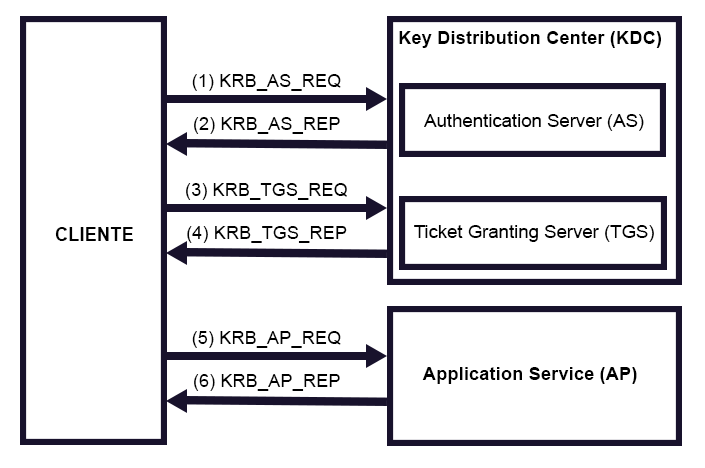
\includegraphics[width=16cm]{Kerberos.png}
\end{center}
\caption{Protocolo de autenticación Kerberos.}
\label{Kerberos}
\end{figure}

\begin{Enumerate}
\item Antes de acceder a un servicio, el c
\end{Enumerate}


























\chapter{Active Directory}
Directotio Activo del inglés {\it Active Directory (AD)}, corresponde a la implementación de un servicio de directorio proporcionado por Microsoft. La finalidad principal de este servicio es la gestión y administración centralizada de los recursos y los usuarios pertenecientes a una red de una empresa u organización. La in\-for\-ma\-ción admisitrada por Active Directory se puede agrupar en tres grupos princiaples: recursos (impresoras), servicios (aplicaciones web, aplicaciones de correo electróncio, bases de datos, etc.) y usuarios (cuentas, credenciales, grupos, etc.). Con esta in\-for\-ma\-ción, es posible crear y adminsitrar dominios, usuarios y todos los objetos englobados dentro de la misma red. En este capítulo se va a introducir los términos generales y conceptos clave y la creación de un laboratorio local que permita la ejecución de los principales ataques sobre Active Directory.

\section{Protocolos y servicios implicados en Active Directory}

\subsubsection{Domain Name System (DNS)}

{\it Domain Name System (DNS)} es el sevicio que proporciona la resolución de nombres de dominio, es decir, resuleve la dirección IP de cada nombre de dominio utilizado en un entorno Active Directory. Este servicio es de gran importancia ya que Active Directory se basa en la resolución de nombres para establecer qué recursos están disponibles a lo largo de una red y dónde se encuentran. 


\subsubsection{Lightweight Directory Access Protocol (LDAP)}

{Lightweight Directory Access Protocol (LDAP)} es un procolo que sirve para acceder a los servicios de directorio. Es utilizado por Active Directory como mecanismo de comunicación entre apliciones y equipos con los servicios que dispone el directorio. Además realiza un seguimiento de los objetos existentes en una red. 


\subsubsection{Server Message Block (SMB)}

{\it Server Message Block (SMB)} es utilizado para el intercambio de archivos a través de un dominio en servicio de Active Directory. Los controladores de dominio utilizan este protocolo para intercambiar Group Policy Objects. 


\section{Términos y conceptos clave}


\subsubsection{Active Directory Domain Services (ADDS)}

{\it Active Directory Domain Services (ADDS)} es el servicio de Active Directory cuando este es intalado en un servidor como por ejemplo Windows Server 2016 ó Windows Server 2019.

\subsubsection{Dominio (Domain)}

Un dominio, del inglés {\it Domain}~\cite{Capitulo4:Domain} es definido como un ``contenedor lógico'', es decir, es una estructura lógica que contiene los siguientes componentes:

\begin{itemize}
\item Una estructura jerárquica para usauarios y grupos en función de los privilegios de los mismos.
\item Servicios (vistos anteriormente) que proveen capacidades de autenticación y autorización.
\item Distintas políticas de seguridad que se aplican a usuarios y objetos.
\item Un registro DNS que identifica inequívocamente el dominio, como puede ser empresa.com, ad.empresa.com. Este nombre será requisito para iniciar sesión en una cuenta de dominio utilizándose como parte del nombre del usuario. 
\end{itemize}

Estos componentes y objetos están almacenados en la base de datos de Active Directory. Se puede considerar un dominio como un límite administrativo de estos objetos. Un dominio puede abarcar diferentes ubicaciones tanto físicas como en red y estar compuesto por una multitud de objetos.

\subsubsection{Árbol (Domain Tree)}

En relación con el término anterior, un árbol del inglés {Domain Tree}, son colecciones de dominios que se agrupan como una estructura jerárquica. Un arbol se le puede considerar como una serie de dominios conectados jerárquicamente a través de usar el mismo espacio de nombres DNS. Un ejemplo sería, si al dominio anterior: empresa.com le añadimos un ``hijo'' denominado recursoshumanos.empresa.com se crea un árbol de dominios compuesto por un dominio padre o root (empresa.com) y un hijo o child (recursoshumanos.empresa.com). Estos dominios forman parte del mismo árbol y se crean automáticamente relaciones de confianza entre ellos. En un Active Directory pueden coexisstir multitud de árboles de dominio diferentes. 

\subsubsection{Bosque (Forest)}
Un bosque, del inglés {\it Forest}, a grandes rasgos es una colección de árboles de dominio que comparten el mismo {\it schema}, misma estructura lógica, {\it global catalog} y configuración. Alguno de estos términos será introducido a continuación. Todos los dominios pertenecientes a un mismo forest, establecen una relación de confianza transitiva. Cabe destacar, que cuando se crea una instacia de Active Directory por primera vez y se crea un dominio también se está creando implícitamente un forest. 

\subsubsection{Schema}

Un {\it schema} en Active Directory se define como a {\it forest-wide template}, es decir, una plantilla aplicable al dominio que define los objetos y propiedades alojados en el Active Directory. Este esquema debe estar bien configurado para evitar comprometer la seguridad de todos los dominios del forest. Para su administración existe un grupo especial denominado {\it Schema Admins} que puede editar y configurar dicho schema. 

\subsubsection{Fully Qualified Domain Name (FQDM)}

Fully Qualified Domain Name (FQDN) es la dirección completa que identifica un host o recurso, este está compuesto por la unión del nombre del host {\it hostname} y el dominio. En el ejemplo anterior, un equipo denominado Cliente01 su FQDN sería Cliente01.empresa.com. 

\subsubsection{Domain Controller (DC)}

Un controlador de dominio, del inglés {\it Domain Controller (DC)}, es la parte fundamental de Active Directory, corresponde a servidores de Windows que contienen la base de datos Active Directory y por lo tanto almacenan toda la información correcpondiente a dominios, domain trees, forests, usuarios, servicieos, etc. 

\subsubsection{Objetos (Objects)}

Todos los elementos alamacenados en una base de datos Active Directory se almacenan en forma de objetos, cada objeto tiene un tipo diferente que le diferencia de otros objetos. Cada objeto almacenado tiene un SID diferente que se utiliza para admitir o denegar el acceso del objeto a un recurso del dominio. Los objetos creados por defecto en cualqueir dominio se pueden agrupar de la siguiente forma: 

\begin{itemize}
\item Unidades organizativas, del inglés {\it Organizational Unit (OU)}. 
\item Usuarios.
\item Ordenadores. 
\item Grupos de usuarios.
\item Contactos.
\item Carpetas compartidas. 
\item Impresoras compartidas.
\end{itemize}

\subsubsection{Organizational Unit (OU)}

Unidades organizativas, del inglés {\it Organizational Unit (OU)} son contenedores de diferentes objetos del mismo dominio como puede ser otros contenedores, cuentas de usuario, grupos, etc. Un administrador del dominio puede crear unidades organizativas y aplicarle diferentes directivas de grupo que se aplicarán a todos los objetos de esta unidad, esto permite una administración más eficiente del Active Directory. 

\subsubsection{Service Principal Name (SPN)}

Un {\it Service Principal Name (SPN)}~\cite{Capitulo4:SPN} es un identificador único asociado a una instacia de un servicio. Los SPN son utilizados por el protocolo de autenticación Kerberos para asociar una instacia de un servicio en concreto con una cuenta de inicio de sesión.  


\section{Laboratorio de Active Directory}

En la siguiente sección se van a establecer las directrices para la creación de un laboratorio local que permita la realización de los ataques que se describirán y expemirentación en los capítulos previos a este. La organización de este capítulo es la siguiente: En primer lugar se detallan los requisitos o prerrequisitos necesarios para poder realizar las siguientes acciones como puede ser el software de virtualización, las imágenes del sistema operativo, etc. Posteriormenente, se ha definido y configurado la topología elegida y por último la instalación y administración de Active Directory. 

\subsection{Requisitos}

Previamente a la creación de la topología de red y a la instalción de  Active Directory que permita realizar las pruebas es necesario disponer de las siguientes características.

\subsubsection{Software de virtualización}

La virtualización consiste en la creación de entornos simulados o recursos desde un único sistema operativo denominado {\it host}, por consecuencia, un software de virtualización es aquel que te permite realizar las acciones descritas anteriormente que puede ser la creación de sistemas operativos, creación de topologías de red, administración de recursos etc. Aunque hay gran variadad de sotfware de virtualización, para la realización de este proyecto se ha utilizado {\it Oracle VM VirtualBox}~\cite{Capitulo4:VirtualBox}.\\

{\it VirtualBox} es un software de virtualización {\it Open Source} con licencia GPLv2 desarrollado por Oracle Corporation que permite la creación de entornos x86 and AMD64/Intel64. Para este proyecto se ha utilizado la última versión (VirtualBox 6.0.12) que se puede desacargar en \footnote{https://www.virtualbox.org/}. Con este Software se van a crear las máquinas virtuales y las redes internas necesarias para la creación del laboratorio. 

\subsubsection{Máquinas Virtuales}

Para este proyecto se van a utilizar cuatro máquinas virtuales. Para aquellas que se necesite una licencia de software privativo se va a utilizar la versión de prueba que proporciona Microsoft con el objetivo de que cualquier pueda replicar dicho laboratorio sin necesidad de lincencias adicionales. Las máquinas son las siguientes:

\begin{itemize}
\item \textbf{DC01}: El la máquina virtual principal y es la encargada de administrar el Active Directory. Como se ha comentado en el estado del arte se va a utilizar Windows Server 2019 es su última versión. La imagen del sistema operativo se ha descargado de \footnote{https://www.microsoft.com/en-us/evalcenter/evaluate-windows-server-2019}.

\item \textbf{Cliente01}: Por otro lado, esta máquina representa a la de un usuario legítimo o cliente de una empresa que está unido al dominio y conectado por la red interna. Para esta máquina virtual se ha utilizado Windows 10 Enterprise que se puede descargar en \footnote{https://www.microsoft.com/en-us/evalcenter/evaluate-windows-server-2019}. 

\item \textbf{Gateway}: Esta máquina virtual se va a utilizar como puerta de enlace entre la red interna y la red externa lo que simula ser internet. Para su implementación, se ha utilizado Debian 10 (Buster) sin escritorio para ahorrar recursos locales. La imagen de este sistema operativo se puede descargar en \footnote{https://cdimage.debian.org/debian-cd/current/amd64/iso-cd/debian-10.1.0-amd64-netinst.iso}.

\item \textbf{Atacante01}: Por último, para la simulación de un atacante externo o profesional de la seguirdad ofensiva realizando labores de {\it Red Team}, se ha utilizado la distribución Kali Linux 2019.3, este distribución ofrece gran variedad de herramientas destinadas a la auditoría informática que serán de utilidad a la hora de realizar los ataques propuestos. Para descargar esta distribución se puede a través de \footnote{https://cdimage.kali.org/kali-2019.3/kali-linux-2019.3-amd64.iso}.

\end{itemize}


\subsubsection{Instalación y actualización}

La instalación y actualización de las máquinas, no se ha considerado como alcance de este proyecto, por lo tantoa partir de este punto se da por hecho de que el usuario ha instalado y actualizado las máquinas y cuenta con la última versión de las mismas. 

\subsection{Configuración previa}

Antes de configurar el active directory, se ha creado una topología en red simula a un entorno coorporativo fictio. Aunque este laboratorio únicamente disponga de una máquina unida al dominio, en entornos reales son multitud los equipos lo que posibilita un gran abanico de posibles entradas a la red de la empresa u organización. A contanuación se va a explicar la topología elegida y las configuraciones necesarias.. 

\subsubsection{Topología de red}

Como ya se ha adalentado, la máquina consta de 4 máquinas: 2 Windows (DC01 y Cliente01) y 2 Linux (Atacante01 y Gateway). La distribución de la topología en red se puede observar en la Figura \ref{Topología}. En la imagen se puede apreciar la existencia de dos redes: ADNET(192.168.0.0/24) formada por los dos dos Sistemas Windows que forman parte del dominio de la empresa fictia y EXTNET(10.10.10.0) que emula en una red interna lo que sería estar expuesto a internet en un entorno real. Ambas redes están enlazadas por el Gateway. 

\begin{figure}[t!] %[ht!] para here [b] para bottom [t] para top
\begin{center}
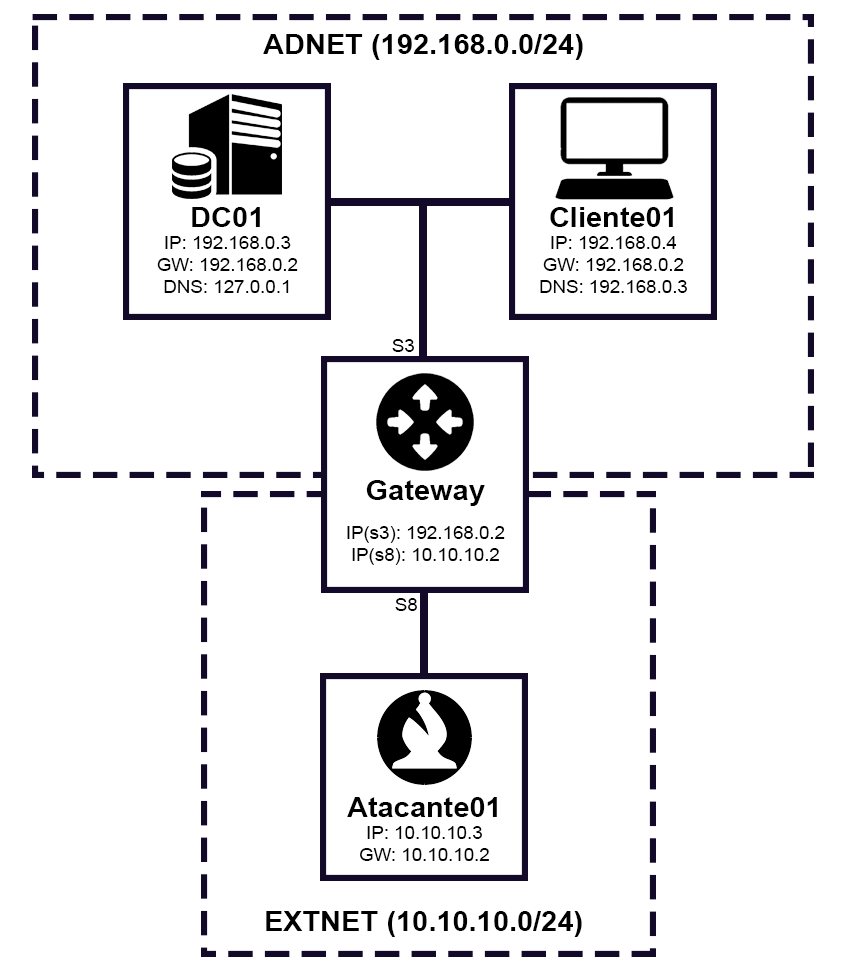
\includegraphics[width=16cm]{Topologia.png}
\end{center}
\caption{Topología del laboratorio local.}
\label{Topología}
\end{figure}

\subsubsection{Configuración de red}

Se va a realizar la configuración necesaria para cada red. 

\begin{itemize}
\item \textbf{DC01}
\begin{enumerate}
\item Antes de arrancar la máquina virtual, es necesario ir a Configuración/Red y añadir el Adaptador1. Esto va a simular la tarjeta de red del DC01. Esta tarjeta de red la vamos a conectar a la red ADNET como se puede ver en la Figura \ref{DC01-Red1}.

\begin{figure}[H] %[ht!] para here [b] para bottom [t] para top
\begin{center}
\includegraphics[width=16cm]{DC01/Red1.png}
\end{center}
\caption{Configuración de red DC01 - Tarjeta de red.}
\label{DC01-Red1}
\end{figure}

\item Una vez iniciada la máquina es necesario dirigirse a {\it Control Panel - Network and Internet - Network Connections} (Figura \ref{DC01-Red2}) y aparecerá la tarjeta de red añadida en el paso anterior. Para editar las direcciones es necesario entrar a las propiedades.
\begin{figure}[H] %[ht!] para here [b] para bottom [t] para top
\begin{center}
\includegraphics[width=16cm]{DC01/Red2.png}
\end{center}
\caption{Configuración de red DC01 - Ajustes de Ethernet.}
\label{DC01-Red2}
\end{figure}

\item Por último, como se puede observar en la Figura \ref{DC01-Red3}, se elige {\it Internet Version Protocol 4(TCP/IPv4) } y después las propiedades de este. Por último, se configura la dirección IP (192.168.0.3), la puerta de enlace correspondiente al Gateway (192.168.0.2) y el DNS. En la mayoría de entornos corporativos es el propio Active Directory el que hace la función de servidor DNS, por lo tanto se escribe la dirección de {\it loopback}: 127.0.0.1.
\begin{figure}[H] %[ht!] para here [b] para bottom [t] para top
\begin{center}
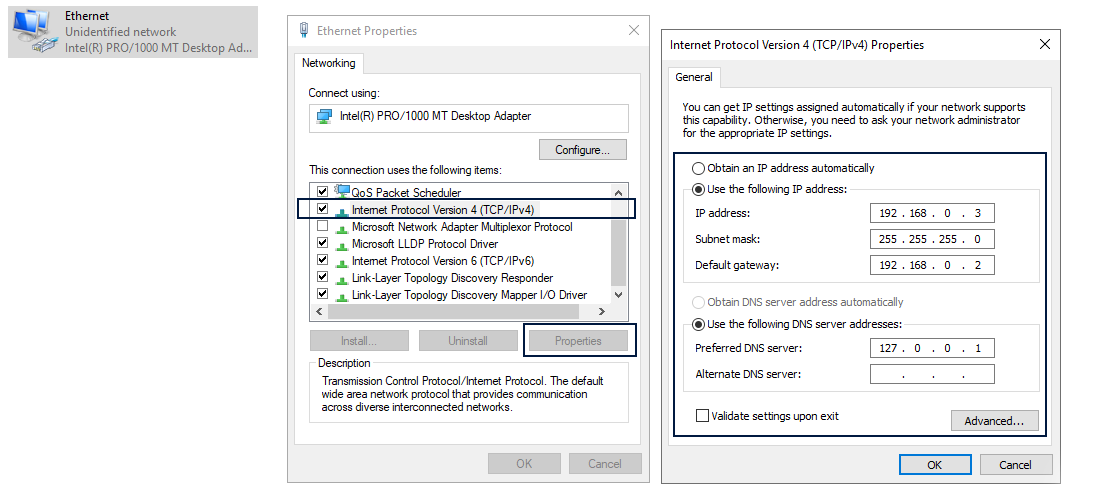
\includegraphics[width=16cm]{DC01/Red3.png}
\end{center}
\caption{Configuración de red DC01 - IPv4.}
\label{DC01-Red3}
\end{figure}
\end{enumerate}

\item \textbf{Cliente01}:
\begin{enumerate}
\item Para configurar la red en el Cliente01, al ser una Máquina Windows en la misma red que el DC01, es necesario repetir los mismos pasos que en la configuración anterior.
\item En el último paso, las direcciones IP son las siguientes: IP(192.168.04) y Gateway(192.168.0.2). En este caso la dirección DNS corresponde a la dirección IP del DC01: 192.168.0.3. La configuración resultante se puede ver en la Figura \ref{Cliente01-Red1}.

\begin{figure}[H] %[ht!] para here [b] para bottom [t] para top
\begin{center}
\includegraphics[width=10cm]{Cliente01/Red1.png}
\end{center}
\caption{Configuración de red Cliente01 - IPv4.}
\label{Cliente01-Red1}
\end{figure}
\end{enumerate}

\item \textbf{Gateway}:

\begin{enumerate}
\item Para esta máquina, es necesario habilitar dos interfaces, una que corresponde a la ADNET o red interna y otra que corresponde con la EXTNET o red externa (Figura \ref{Gateway-Red1}).
\begin{figure}[H] %[ht!] para here [b] para bottom [t] para top
\begin{center}
\includegraphics[width=10cm]{Gateway/Red1.png}
\end{center}
\caption{Configuración de red Gateway - Tarjetas de red.}
\label{Gateway-Red1}
\end{figure}

\item Iniciamos la máquina y comprobamos que se han creado ambas interfaces {\it enp0s3} para la ADNET y {\it enp0s8} para la EXTNET. 

\item A continuación introducimos los siguientes comandos, estos comandos levantan ambas interfaces y asignan las direcciones IP correspondientes. 
\begin{listing}[style=consola, numbers=none]
# ip link set enp0s3 up
# ip a add 192.168.0.2/24 dev enp0s3
# ip link set enp0s8 up
# ip a add 10.10.10.2/24 dev enp0s8
\end{listing}

\item Por último, permitimos que el gateway reenvíe los paquetes que le llegan, para eso se utiliza el siguiente comando: 
\begin{listing}[style=consola, numbers=none]
# echo 1 > /proc/sys/net/ipv4/ip_forward
\end{listing}

\item La configuración final de la máquina se puede observar en la Figura \ref{Gateway-Red2}.
\begin{figure}[H] %[ht!] para here [b] para bottom [t] para top
\begin{center}
\includegraphics[width=15cm]{Gateway/Red2.png}
\end{center}
\caption{Configuración de red Gateway}
\label{Gateway-Red2}
\end{figure}
\end{enumerate}

\item \textbf{Atacante01}:

\begin{enumerate}

\item Esta máquina está en la red externa, por lo tanto añadimos un adaptador de red unida a la red externa (Figura \ref{Atacante01-Red1}). 
\begin{figure}[H] %[ht!] para here [b] para bottom [t] para top
\begin{center}
\includegraphics[width=10cm]{Atacante01/Red1.png}
\end{center}
\caption{Configuración de red Atacante01 - Tarjeta de red}
\label{Atacante01-Red1}
\end{figure}

\item De la misma manera que en el gateway configuramos la interfaz de red, que en este caso es {\it eth0} con los siguientes comandos. 
\begin{listing}[style=consola, numbers=none]
# ip link set eth0 up
# ip a add 10.10.10.3 dev eth0 
\end{listing}

\item Para poder alcazar la red interna, es necesario definir a la dirección 10.10.10.2 como fateway, para que cuando la máquina no encuentre una dirección IP la redirija por ese Gateway. Para ello, se utiliza el siguiente comando: 

\begin{listing}[style=consola, numbers=none]
# ip route default via 10.10.10.2
\end{listing}

\end{enumerate}
\end{itemize}

\subsubsection{Comprobación de la conectividad}

\begin{itemize}

\item \textbf{Cliente01 - DC01}: Para comprobar la conectividad entre Cliente01 y DC10, podemos realizar un ping desde Cliente01 a la dirección IP de DC01 (\ref{Cliente01-Red2}).
\begin{figure}[H] %[ht!] para here [b] para bottom [t] para top
\begin{center}
\includegraphics[width=10cm]{Cliente01/Red2.png}
\end{center}
\caption{Conexión entre Cliente01 y DC01}
\label{Cliente01-Red2}
\end{figure}

\item \textbf{Atacante01 - DC01}: Para comprobar la conectividad dentre Atacante01 y DC10, en vez de realizar un ping intentamos conectarnos a través de Samba (\ref{Atacante01-Red2})
\begin{figure}[H] %[ht!] para here [b] para bottom [t] para top
\begin{center}
\includegraphics[width=10cm]{Atacante01/Red2.png}
\end{center}
\caption{Conexión entre Atacante01 y DC01}
\label{Atacante01-Red2}
\end{figure}

\end{itemize}

\subsubsection{Cambio de nombre del sistema}

Una buena práctica es cambiar el nombre a los Sistemas Windows, esto nos facilitará su identificación y su futura administración. 

\begin{itemize}
\item Para cambiar el nombre a DC01, se puede realizar desde el propio panel de administración del servidor, a través de la opción {\it Local Name Server - Computer Name - Change} como se puede ver en la Figura \ref{DC01-Name1}
\begin{figure}[H] %[ht!] para here [b] para bottom [t] para top
\begin{center}
\includegraphics[width=15cm]{DC01/Name1.png}
\end{center}
\caption{Cambio de nombre DC01}
\label{DC01-Name1}
\end{figure}

\item Para cambiar el nombre a Cliente01, se realiza a través de {\it Control Panel - System and Security - System} posteriormente se elige la opción {\it Change Settings - Change} y se introduce el nombre Cliente01 (\ref{Cliente01-Name1}). Ambos cambios nos van a pedir un reinicio del equipo.  
\begin{figure}[H] %[ht!] para here [b] para bottom [t] para top
\begin{center}
\includegraphics[width=15cm]{Cliente01/Name1.png}
\end{center}
\caption{Cambio de nombre Cliente01}
\label{Cliente01-Name1}
\end{figure}

\end{itemize}

\subsection{Creación y configuración del Active Directory}

En esta sección se va a detallar la instalación y configuración de Active Directory en Windows Server 2019 en la máquina virtual DC01.

\subsubsection{Intalación y configuración}

\begin{enumerate}

\item La instalación de un AD DS se puede realizar desde el Dashboard integrado en Windows Server 2019. Para ello, se selecciona {\it Add roles and features} (Figura \ref{DC01-AD1}).
\begin{figure}[H] %[ht!] para here [b] para bottom [t] para top
\begin{center}
\includegraphics[width=15cm]{DC01/AD1.png}
\end{center}
\caption{Instalación de AD DS - Add roles and features.}
\label{DC01-AD1}
\end{figure}


\item Para el tipo de instalación se va a elegir {\it Roled-based or feature-based installation} (Figura \ref{DC01-AD2}).
\begin{figure}[H] %[ht!] para here [b] para bottom [t] para top
\begin{center}
\includegraphics[width=15cm]{DC01/AD2.png}
\end{center}
\caption{Instalación de AD DS - Roled-based installation.}
\label{DC01-AD2}
\end{figure}


\item Después elegimos el DC01 (O el nombre que se haya elegido al cambiar el nombre en la sección anterior) como se puede ver en la Figura \ref{DC01-AD3}.
\begin{figure}[H] %[ht!] para here [b] para bottom [t] para top
\begin{center}
\includegraphics[width=15cm]{DC01/AD3.png}
\end{center}
\caption{Instalación de AD DS - DC01.}
\label{DC01-AD3}
\end{figure}


\item En la sección {\it Server Roles} se elige Active Directory Domain Services (Figura \ref{DC01-AD4}), al seleccionar esta opción se desplegará un menú donde debemos especifiar las caracterísitcas, se seleciona en {\it Add Features}.
\begin{figure}[H] %[ht!] para here [b] para bottom [t] para top
\begin{center}
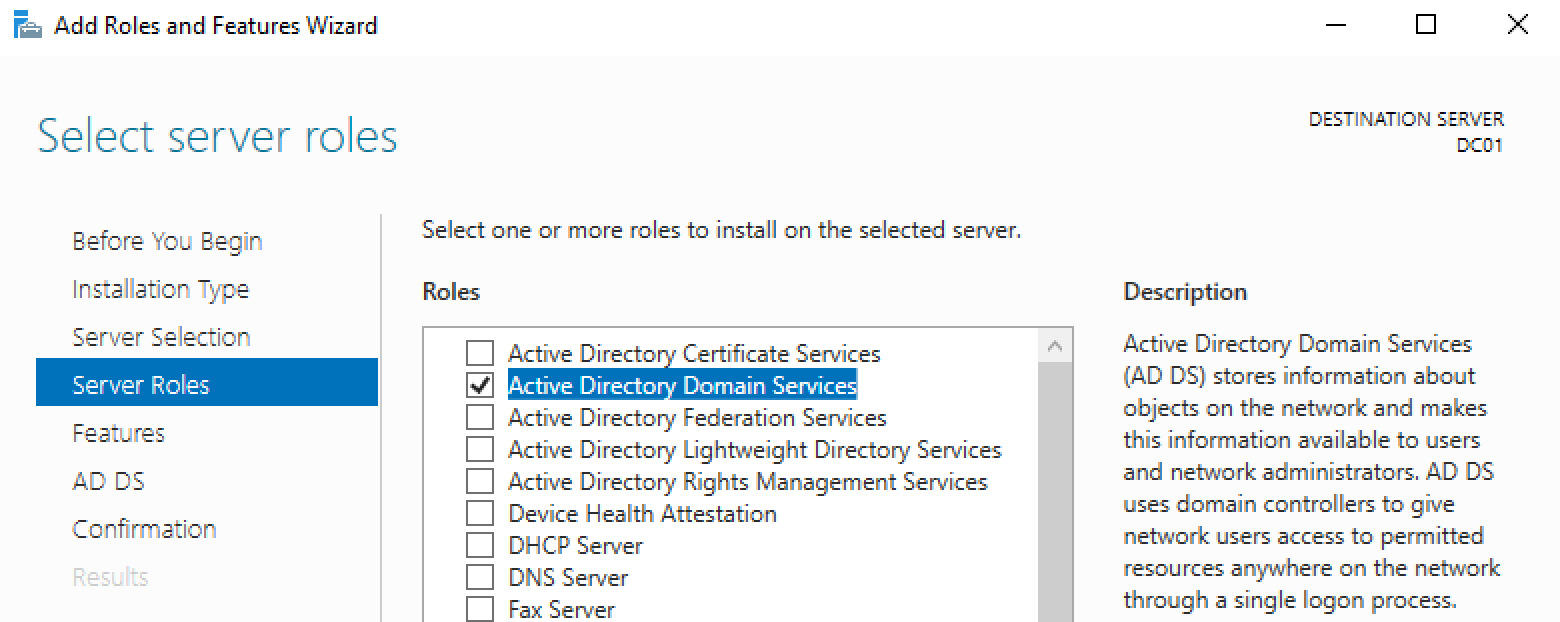
\includegraphics[width=15cm]{DC01/AD4.png}
\end{center}
\caption{Instalación de AD DS - Active Directory Domain Services.}
\label{DC01-AD4}
\end{figure}


\item Después seguimos la instalción hasta la opción {\it Confirmation} e instalamos AD DS (Figura \ref{DC01-AD5}).
\begin{figure}[H] %[ht!] para here [b] para bottom [t] para top
\begin{center}
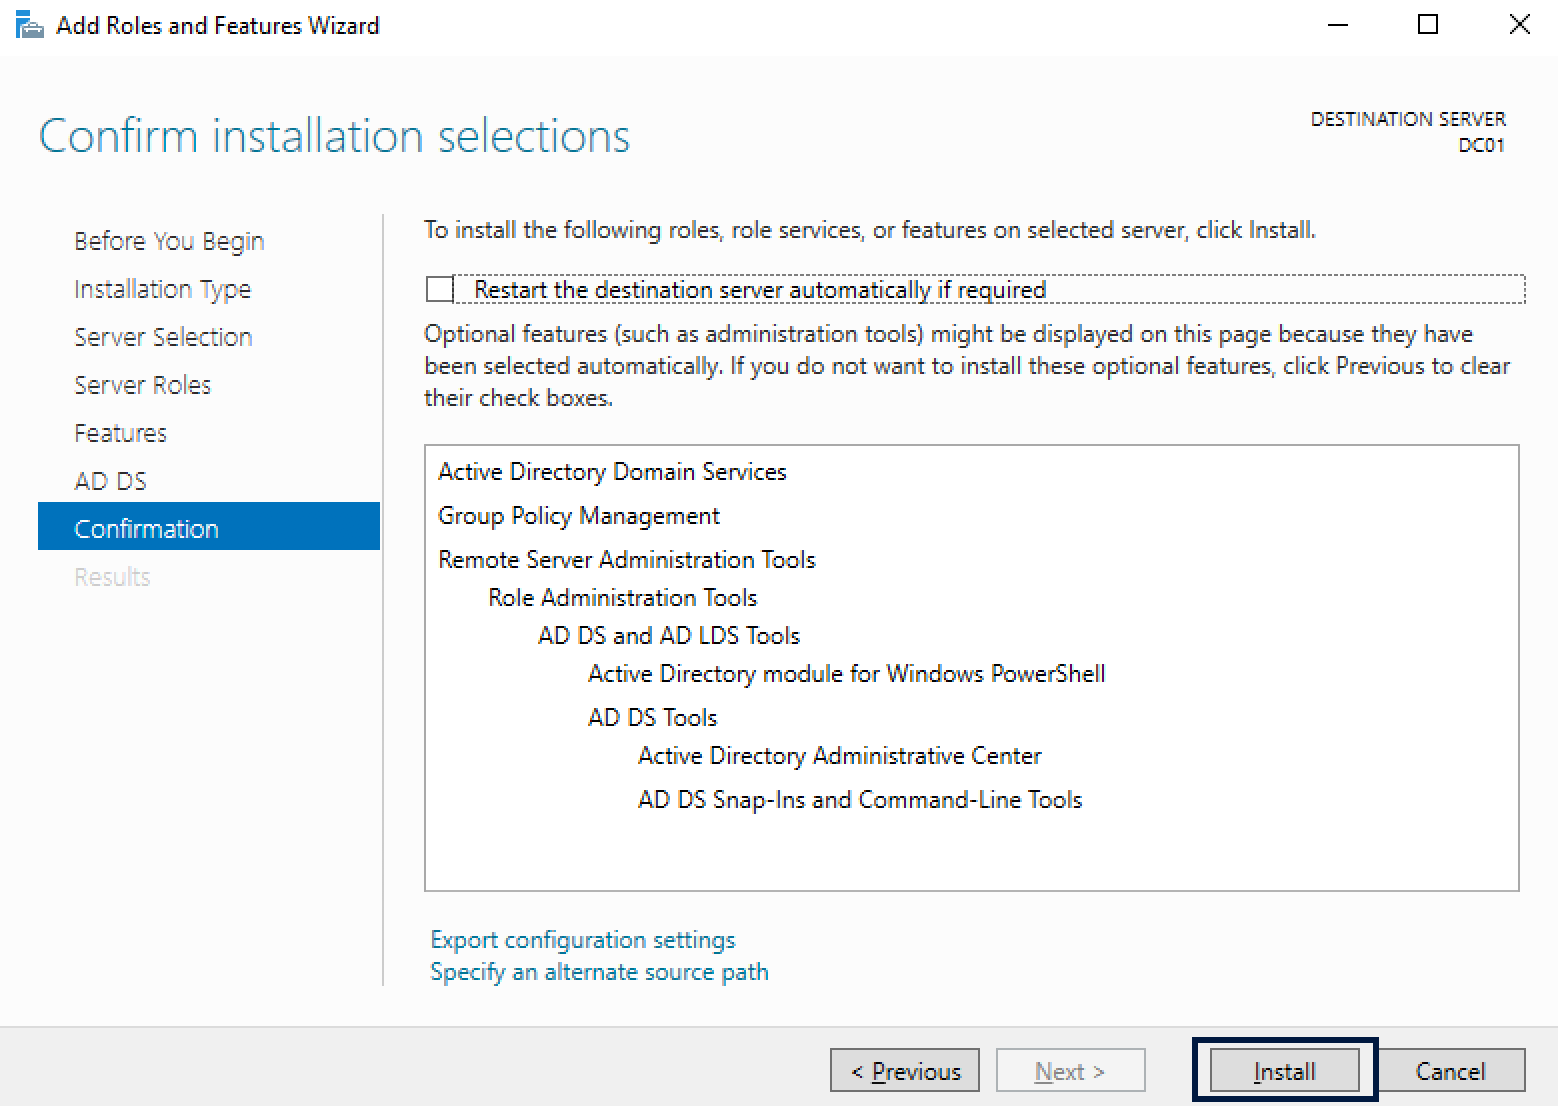
\includegraphics[width=15cm]{DC01/AD5.png}
\end{center}
\caption{Instalación de AD DS - Instalación.}
\label{DC01-AD5}
\end{figure}


\item Cuando se termina la instlación se debe ``promocionar'' el servidor DC01 como Domain Controller, para ello seleccionamos la opción que se puede ver en la Figura \ref{DC01-AD6}.
\begin{figure}[H] %[ht!] para here [b] para bottom [t] para top
\begin{center}
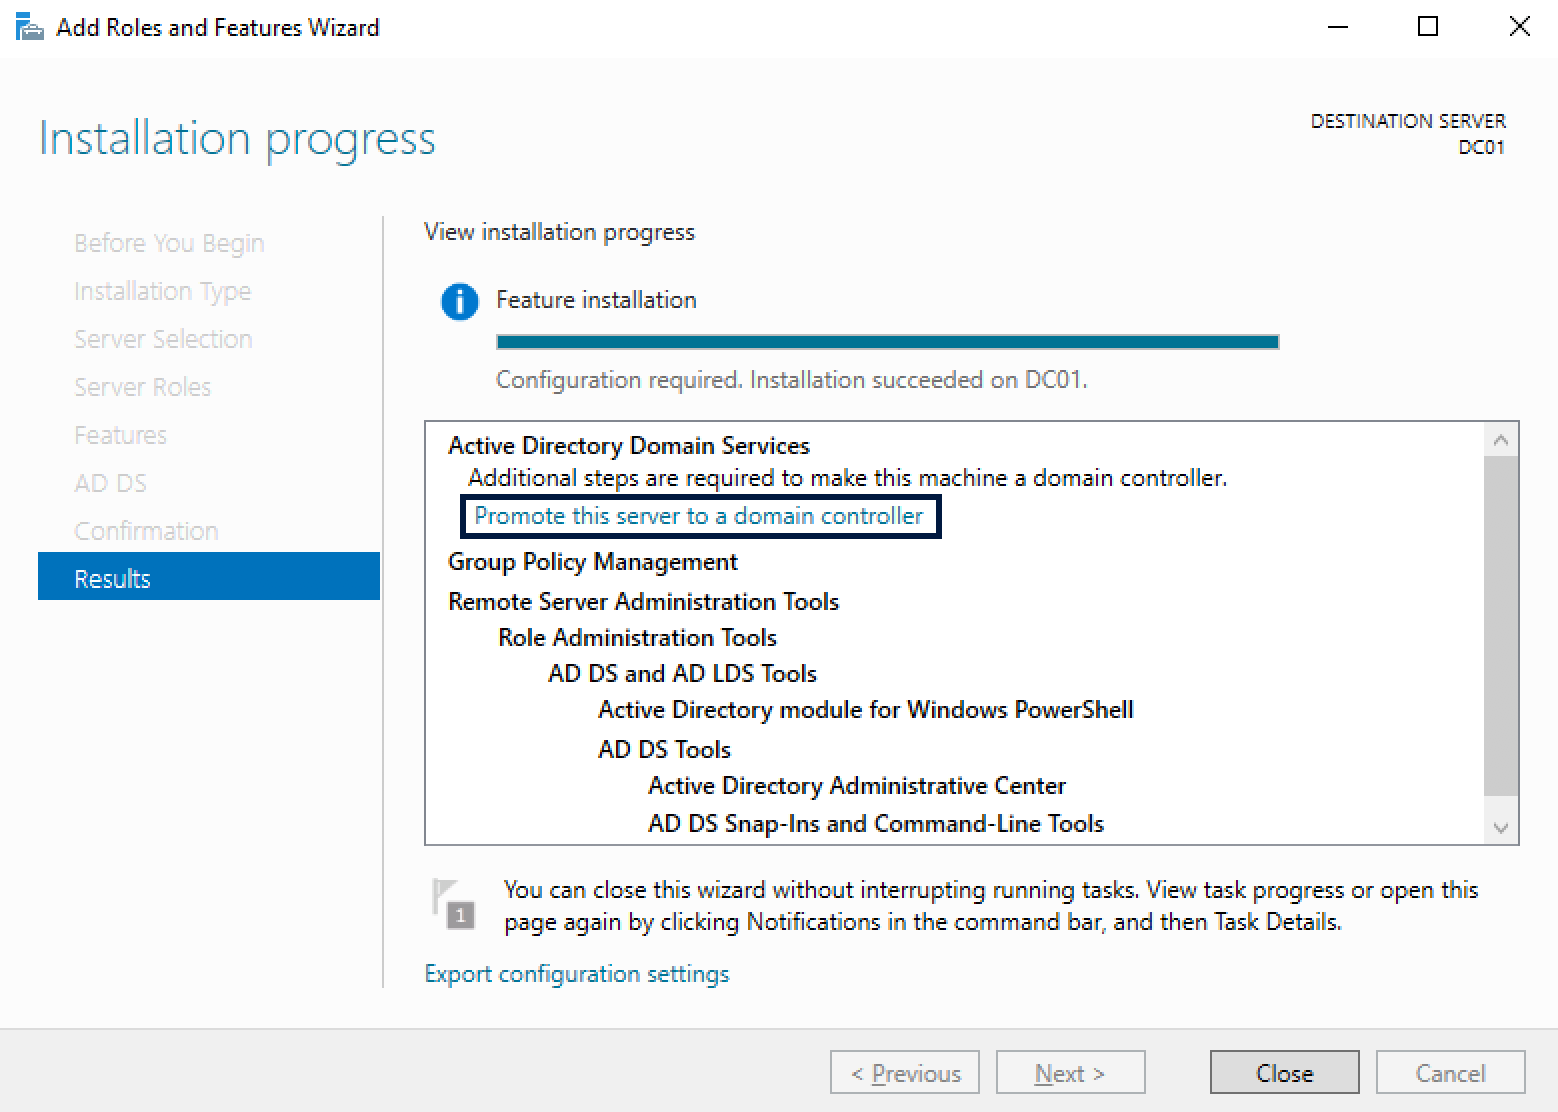
\includegraphics[width=15cm]{DC01/AD6.png}
\end{center}
\caption{Instalación de AD DS - Promote to Domain Controller.}
\label{DC01-AD6}
\end{figure}


\item Posteriormente, al no disponer de ningún forest previo, es necesario crear uno con el nombre {\it laboratory.com} (Figura \ref{DC01-AD7}). 
\begin{figure}[H] %[ht!] para here [b] para bottom [t] para top
\begin{center}
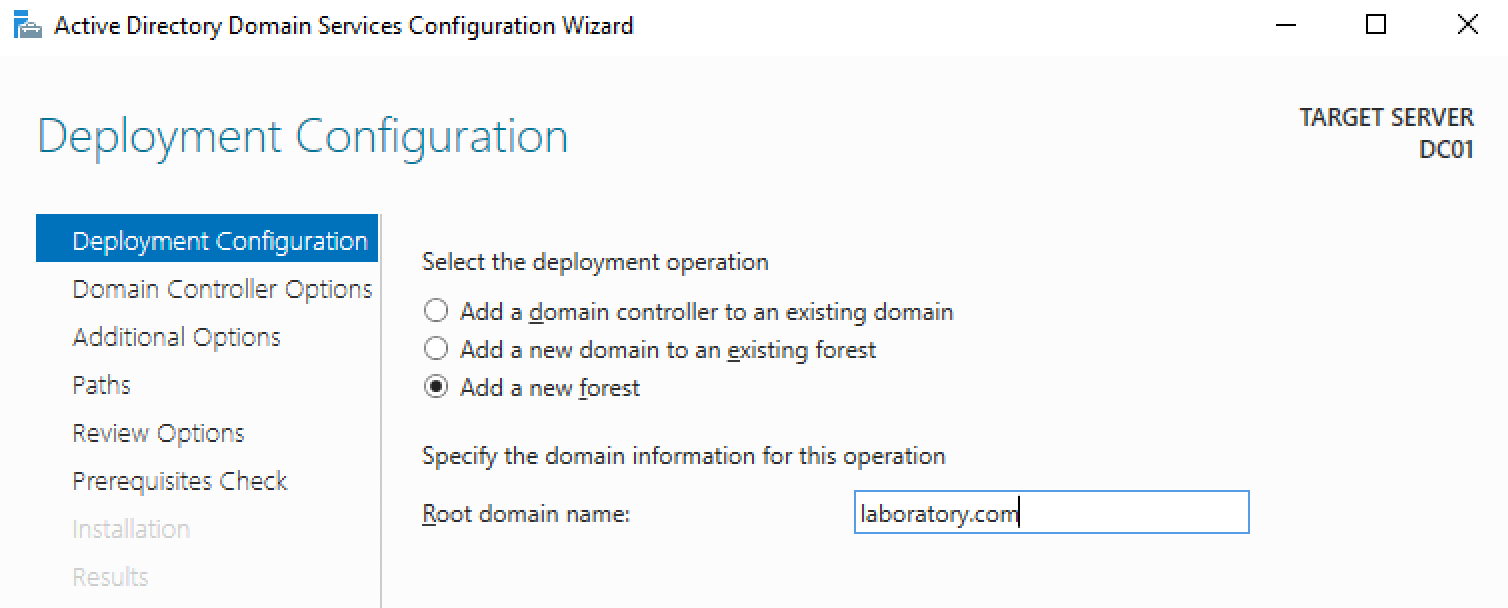
\includegraphics[width=15cm]{DC01/AD7.png}
\end{center}
\caption{Instalación de AD DS - Creación del forest laboratory.com.}
\label{DC01-AD7}
\end{figure}


\item En la pestaña {\it Domain Controller Options} elegimos Windows Server 2016 al ser la versión más actualizada posible, después si no se dispone de un DNS externo, se elige que el Domain Controllertenga la capacidad de DNS y Global Catalog. Además, se elige la contraseña para el Directory Services Restore Mode (DSRM) (Figura \ref{DC01-AD8}).
\begin{figure}[H] %[ht!] para here [b] para bottom [t] para top
\begin{center}
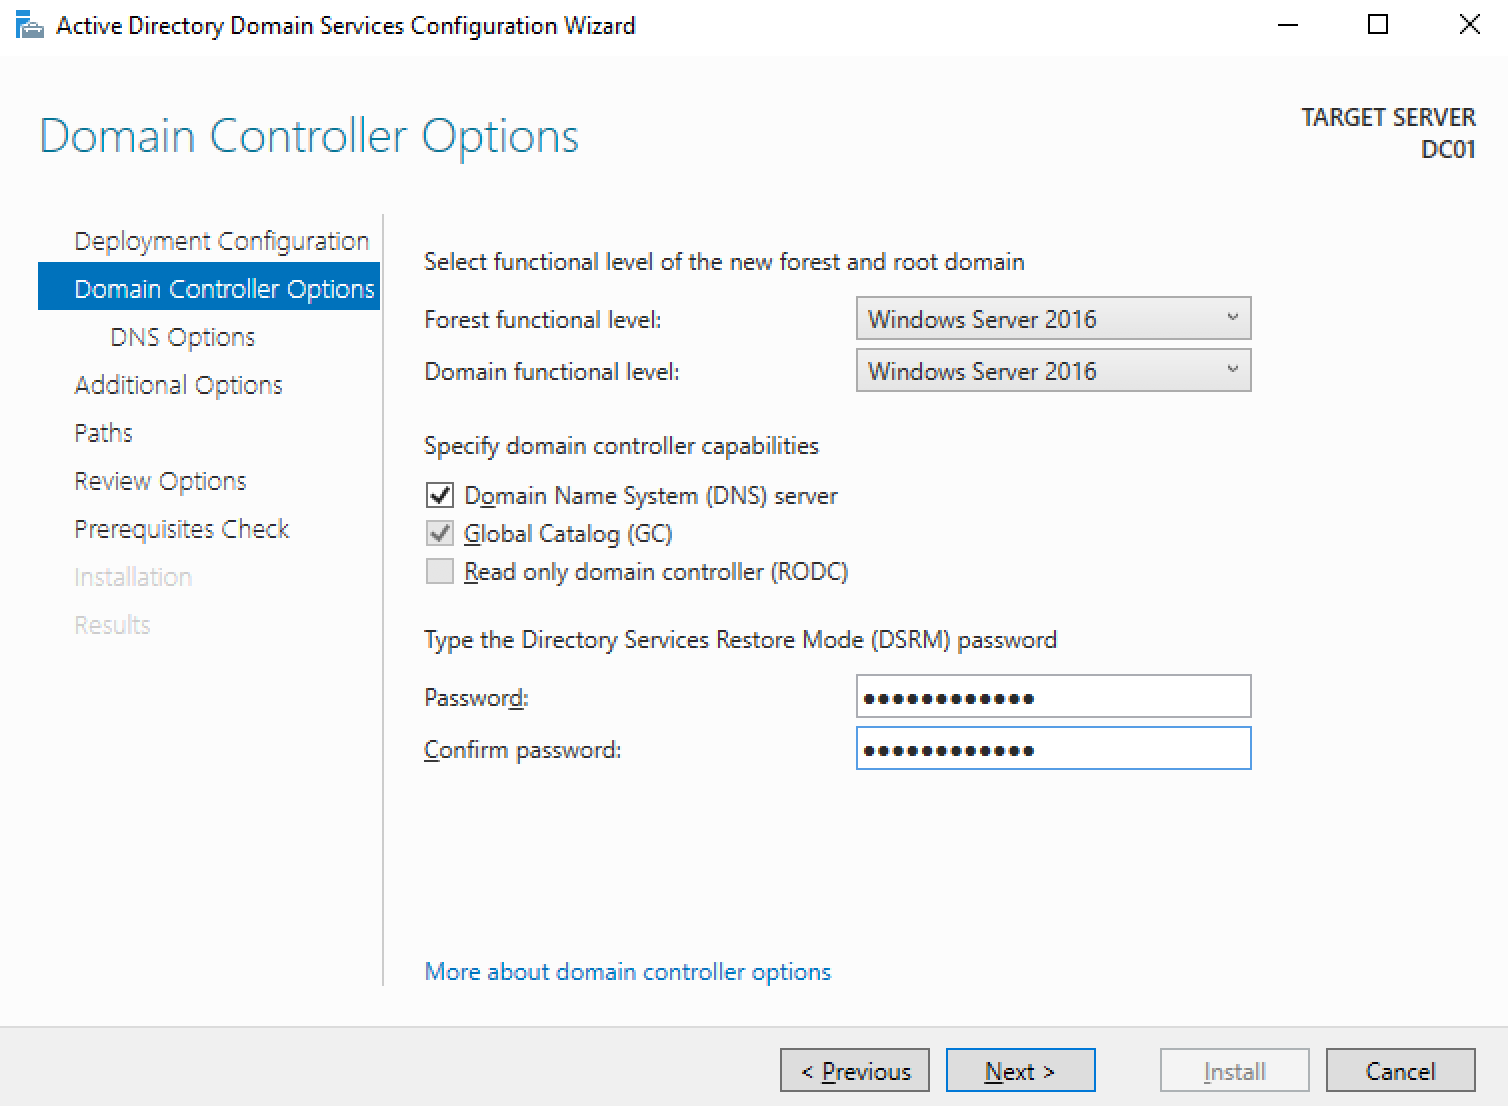
\includegraphics[width=15cm]{DC01/AD8.png}
\end{center}
\caption{Instalación de AD DS - Domain Controller options.}
\label{DC01-AD8}
\end{figure}


\item En la pestaña de {\it Paths} podemos ver las rutas de los principales elementos del DC como puede ser la base de datos NTDS y la carpeta SYSVOL (Figura \ref{DC01-AD9}).
\begin{figure}[H] %[ht!] para here [b] para bottom [t] para top
\begin{center}
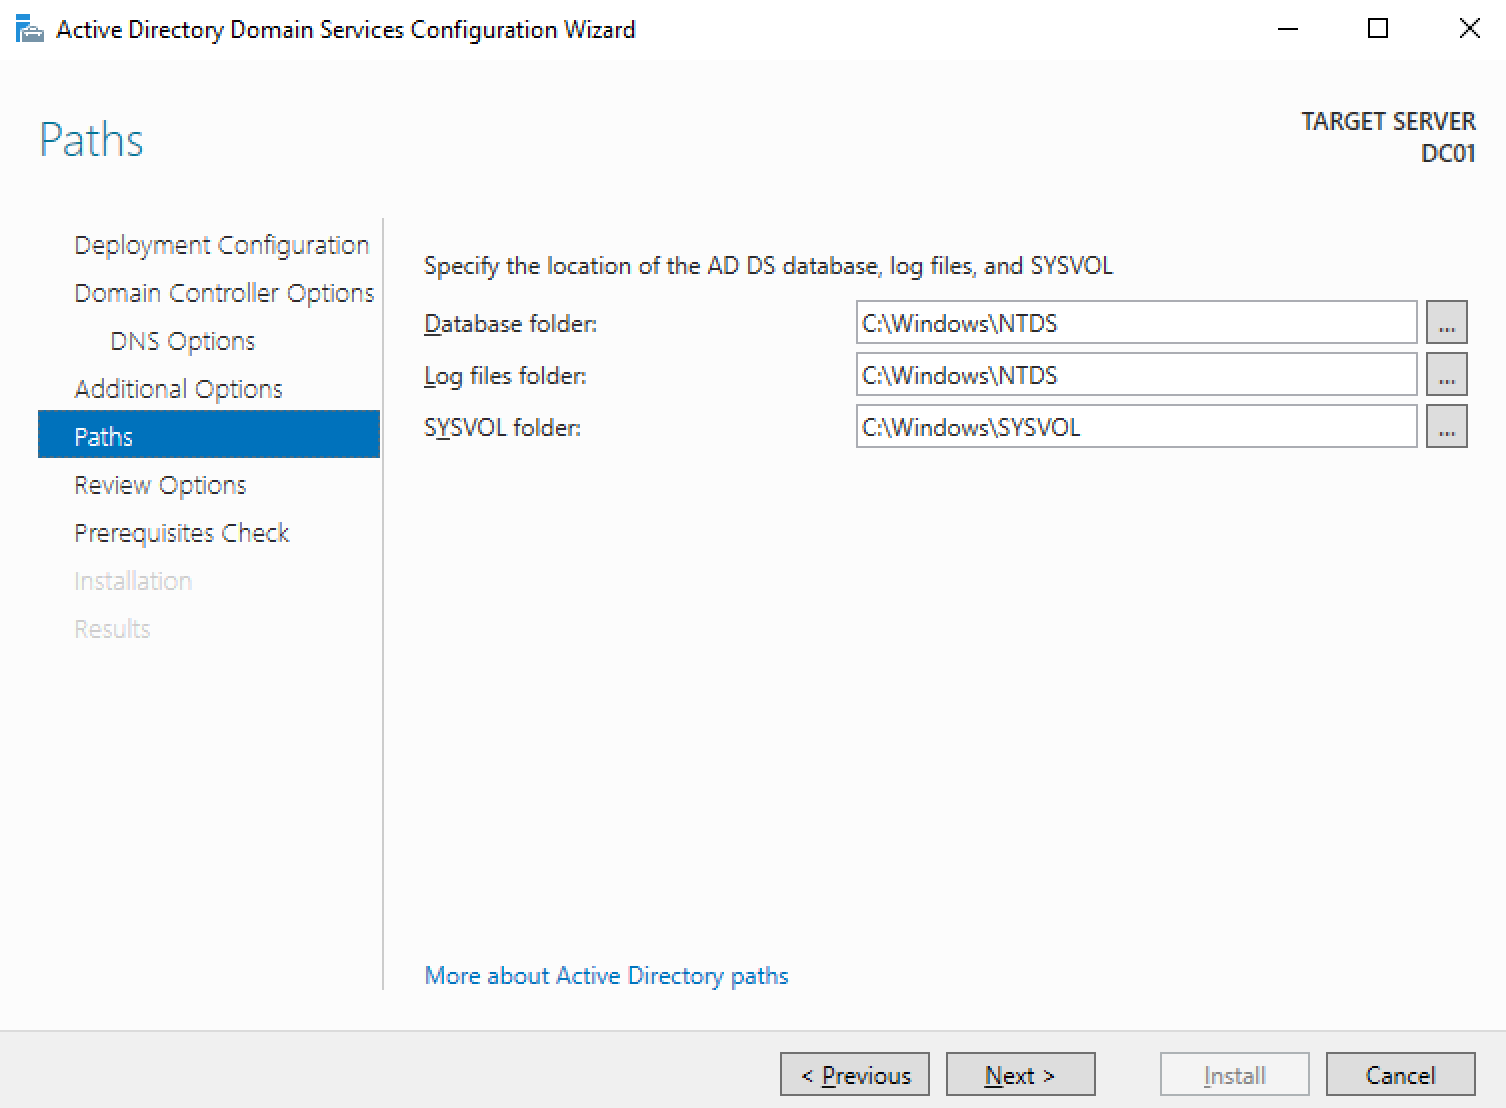
\includegraphics[width=15cm]{DC01/AD9.png}
\end{center}
\caption{Instalación de AD DS - Rutas NTDS y SYSBOL.}
\label{DC01-AD9}
\end{figure}

\item Por último, instalamos las opciones definidas anteriormente Figura \ref{DC01-AD10}. Después de esta opción es necesario reiniciar el servidor. 
\begin{figure}[H] %[ht!] para here [b] para bottom [t] para top
\begin{center}
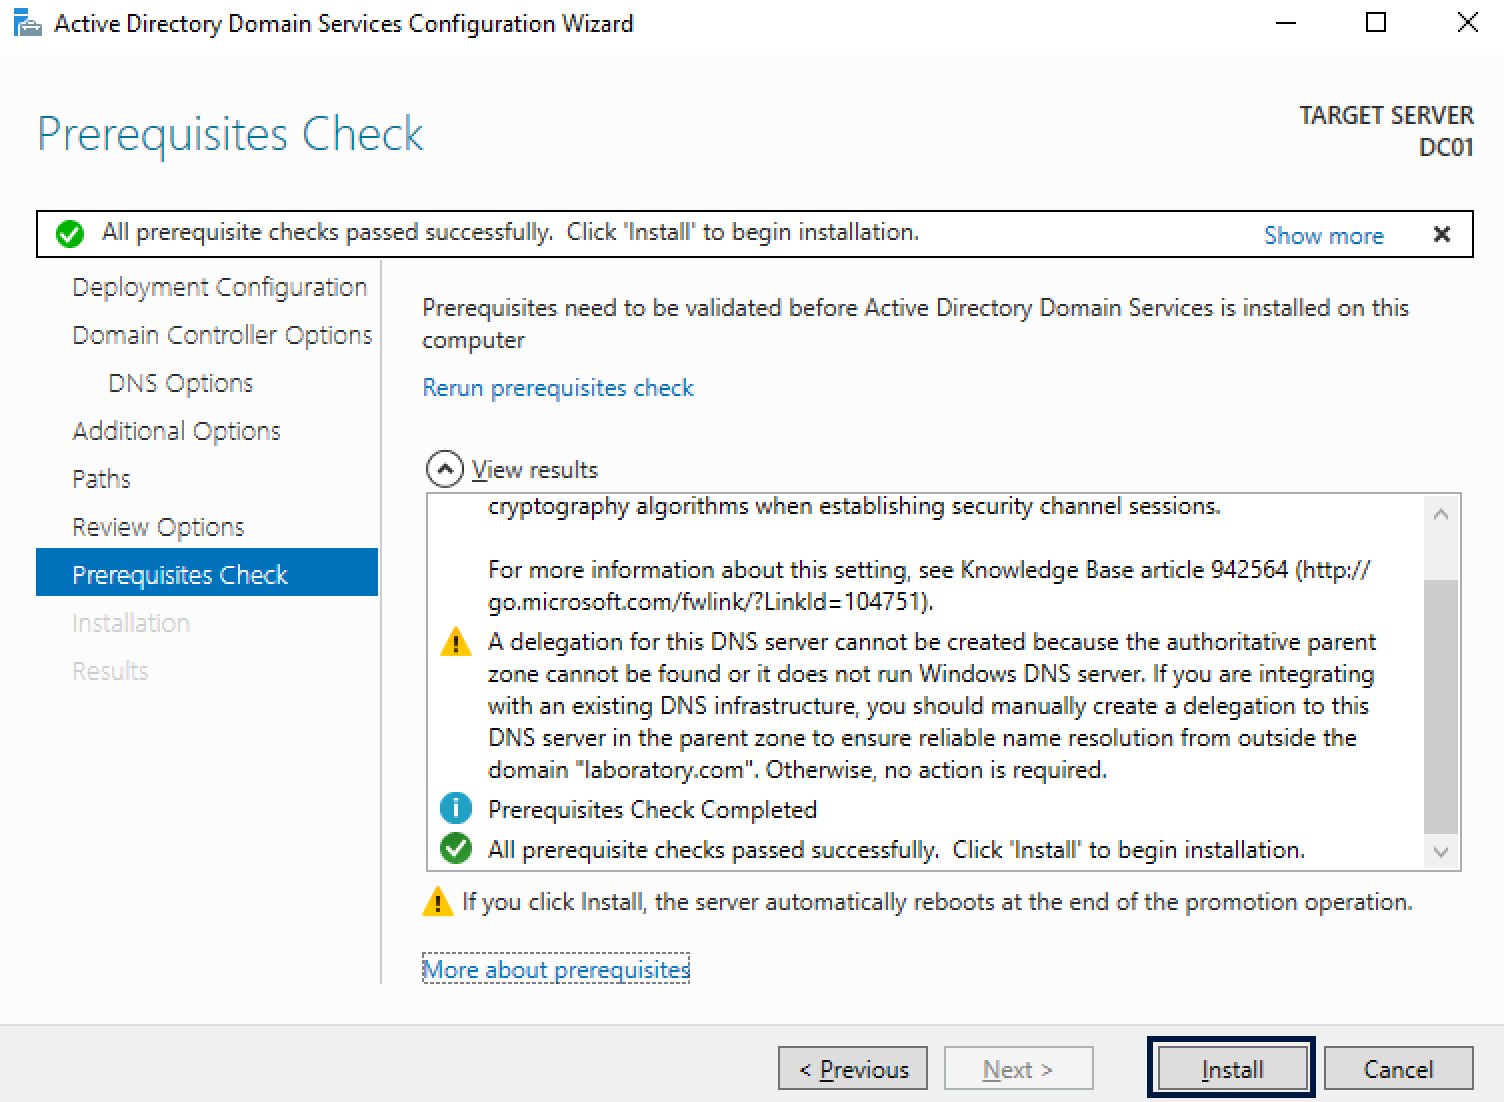
\includegraphics[width=15cm]{DC01/AD10.png}
\end{center}
\caption{Instalación de AD DS - Instalación.}
\label{DC01-AD10}
\end{figure}

\end{enumerate}

\subsubsection{Enlazar cliente al dominio}

Para añadir Cliente01 al dominio {\it laboratory.com} es necesario realizar los siguientes pasos: 

\begin{enumerate}
\item Del mismo modo que para cambiar el nombre al equipo, es necesario ir a {\it Control Panel - System and Security - System}, después realizar click en {\it Change settings} (Figura \ref{Cliente01-AD1}). 
\begin{figure}[H] %[ht!] para here [b] para bottom [t] para top
\begin{center}
\includegraphics[width=15cm]{Cliente01/AD1.png}
\end{center}
\caption{Enlazar cliente al dominio - Settings.}
\label{Cliente01-AD1}
\end{figure}

\item Después se selecciona {\it change} y en la opción de {\it Member of - Domain} se elige el dominio {\it laboratory.com} (Figura \ref{Cliente01-AD2}).
\begin{figure}[H] %[ht!] para here [b] para bottom [t] para top
\begin{center}
\includegraphics[width=15cm]{Cliente01/AD2.png}
\end{center}
\caption{Enlazar cliente al dominio - Dominio.}
\label{Cliente01-AD2}
\end{figure}


\item Al confirmar este cambio se requiere las credenciales del Domain Admin (Figura \ref{Cliente01-AD3}) y reiniciar el sistema.
\begin{figure}[H] %[ht!] para here [b] para bottom [t] para top
\begin{center}
\includegraphics[width=15cm]{Cliente01/AD3.png}
\end{center}
\caption{Enlazar cliente al dominio - Log on.}
\label{Cliente01-AD3}
\end{figure}

\item Finalmente, se puede confirmar que la operación se ha realizado correctamente desde el DC01 desde la opción {\it Tools - Active Directory Users and Computers - Laboratory.com - Computers} (Figura \ref{DC01-AD12}) del Dashboard como se puede ver en la Figura \ref{DC01-AD11}. 
\begin{figure}[H] %[ht!] para here [b] para bottom [t] para top
\begin{center}
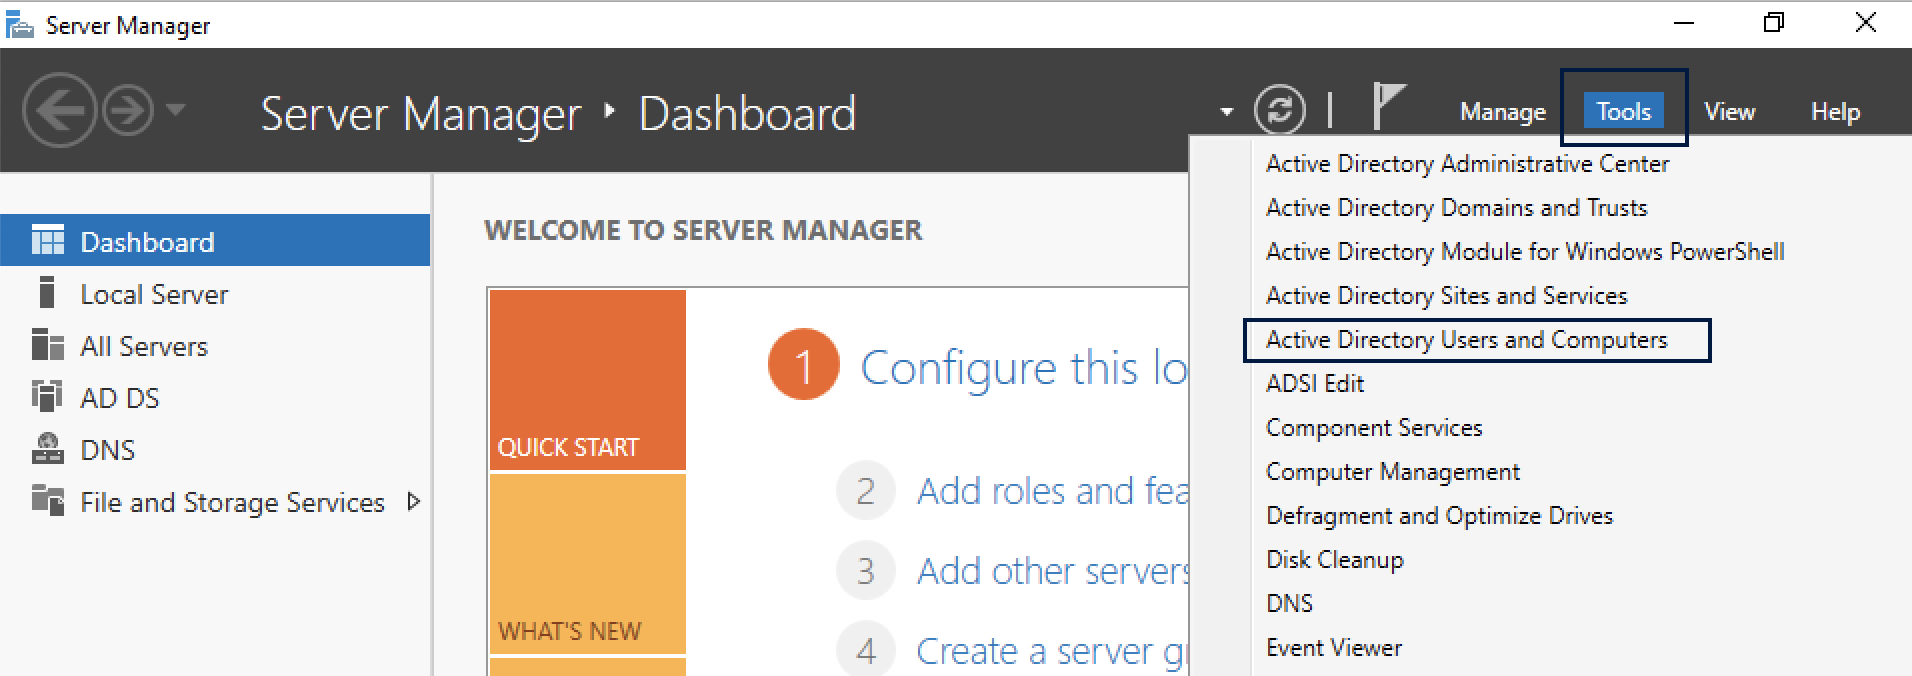
\includegraphics[width=15cm]{DC01/AD12.png}
\end{center}
\caption{Enlazar cliente al dominio - Users and Computers.}
\label{DC01-AD12}
\end{figure}

\begin{figure}[H] %[ht!] para here [b] para bottom [t] para top
\begin{center}
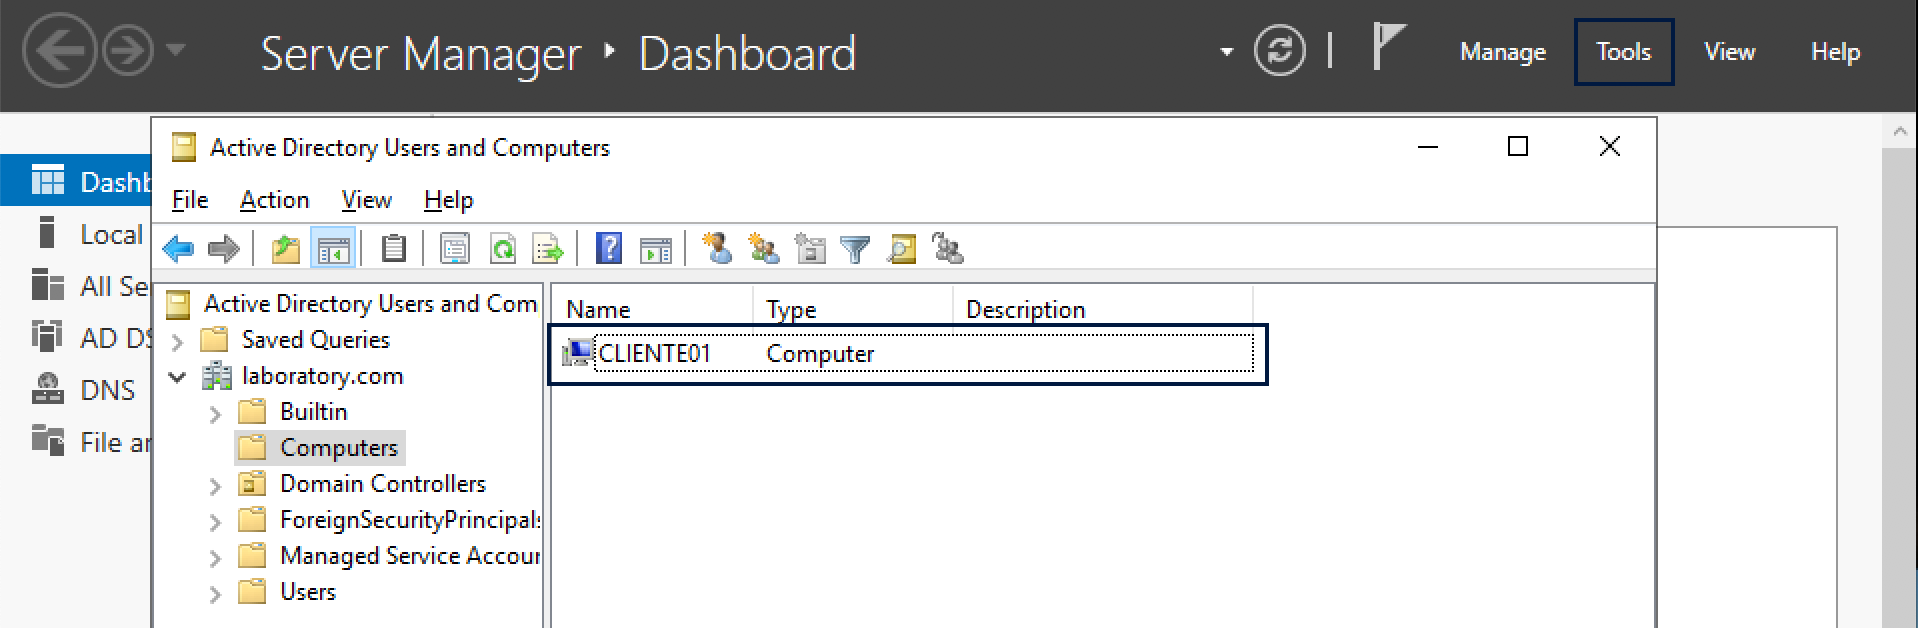
\includegraphics[width=15cm]{DC01/AD11.png}
\end{center}
\caption{Enlazar cliente al dominio - Dashboard.}
\label{DC01-AD11}
\end{figure}


\end{enumerate}

\subsubsection{Creación de usuarios}

Para la fase de experimentación, además, se van a crear tres usuarios con distintos privilegios de administración en el dominio. Para ello, desde DC01 se elige la opción {\it Tools - Active Directory Users and Computers - Laboratory.com - Computers} (Figura \ref{DC01-AD12}) y después se selecciona {\it Users - New - User} como el la Figura \ref{DC01-AD13}. 

\begin{figure}[H] %[ht!] para here [b] para bottom [t] para top
\begin{center}
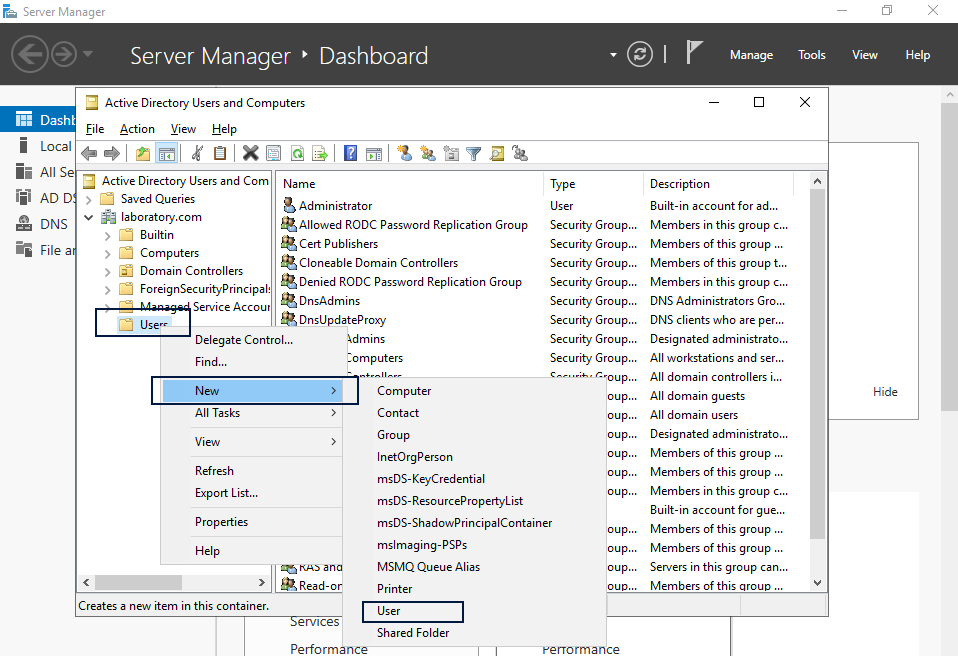
\includegraphics[width=15cm]{DC01/AD13.png}
\end{center}
\caption{Crear nuevo usuario.}
\label{DC01-AD13}
\end{figure}

\begin{itemize}

\item Usuario de dominio (Figura \ref{DC01-User1}). 
\begin{figure}[H] %[ht!] para here [b] para bottom [t] para top
\begin{center}
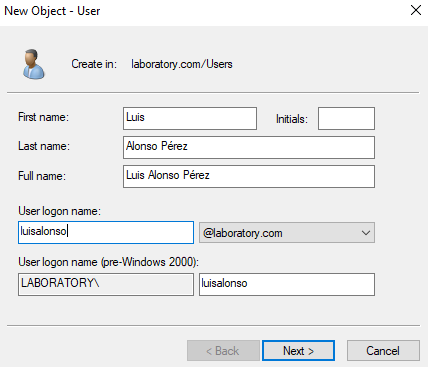
\includegraphics[width=10cm]{DC01/User1.png}
\end{center}
\caption{Usario de dominio.}
\label{DC01-User1}
\end{figure}


\item Usuario de dominio y administrador del dominio (Figura \ref{DC01-User1}). 
\begin{figure}[H] %[ht!] para here [b] para bottom [t] para top
\begin{center}
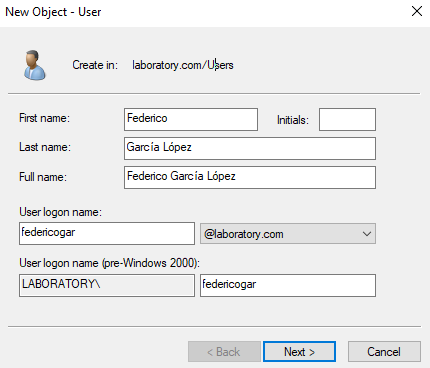
\includegraphics[width=10cm]{DC01/User2.png}
\end{center}
\caption{Usuario de dominio y administrador del dominio.}
\label{DC01-User2}
\end{figure}

Para añadirlo al grupo de administradores de dominio, seleccionamos la opción {\it Add to a group...} (Figura \ref{DC01-User3}).

\begin{figure}[H] %[ht!] para here [b] para bottom [t] para top
\begin{center}
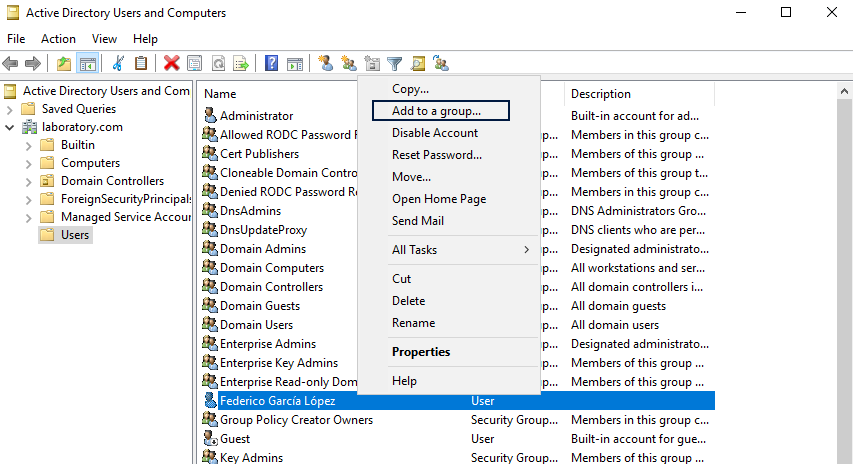
\includegraphics[width=10cm]{DC01/User3.png}
\end{center}
\caption{Añadir el usuario a un grupo.}
\label{DC01-User3}
\end{figure}

Y se añade el grupo {\it Domain Admins} (Figura \ref{DC01-User4}).

\begin{figure}[H] %[ht!] para here [b] para bottom [t] para top
\begin{center}
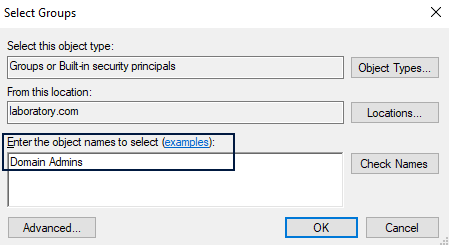
\includegraphics[width=10cm]{DC01/User4.png}
\end{center}
\caption{Grupo Domain Admins.}
\label{DC01-User4}
\end{figure}

\item Usuario de dominio y administrador local en Cliente01 (Figura \ref{DC01-User5}).
\begin{figure}[H] %[ht!] para here [b] para bottom [t] para top
\begin{center}
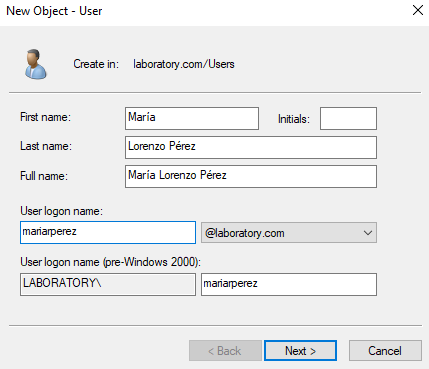
\includegraphics[width=10cm]{DC01/User5.png}
\end{center}
\caption{Usuario de dominio y administrador local.}
\label{DC01-User5}
\end{figure}

Desde una consola con privilegios de administrador local en el Cliente01 ejecutamos el siguiente comando que añade al grupo de administradores el usuario creado previamente. 

\begin{listing}[style=consola, numbers=none]
# net localgroup administrators laboratory\mariarperez /add
\end{listing}

Una vez añadido, es posible loguearse con dicha información (Figura \ref{DC01-User6}).

\begin{figure}[H] %[ht!] para here [b] para bottom [t] para top
\begin{center}
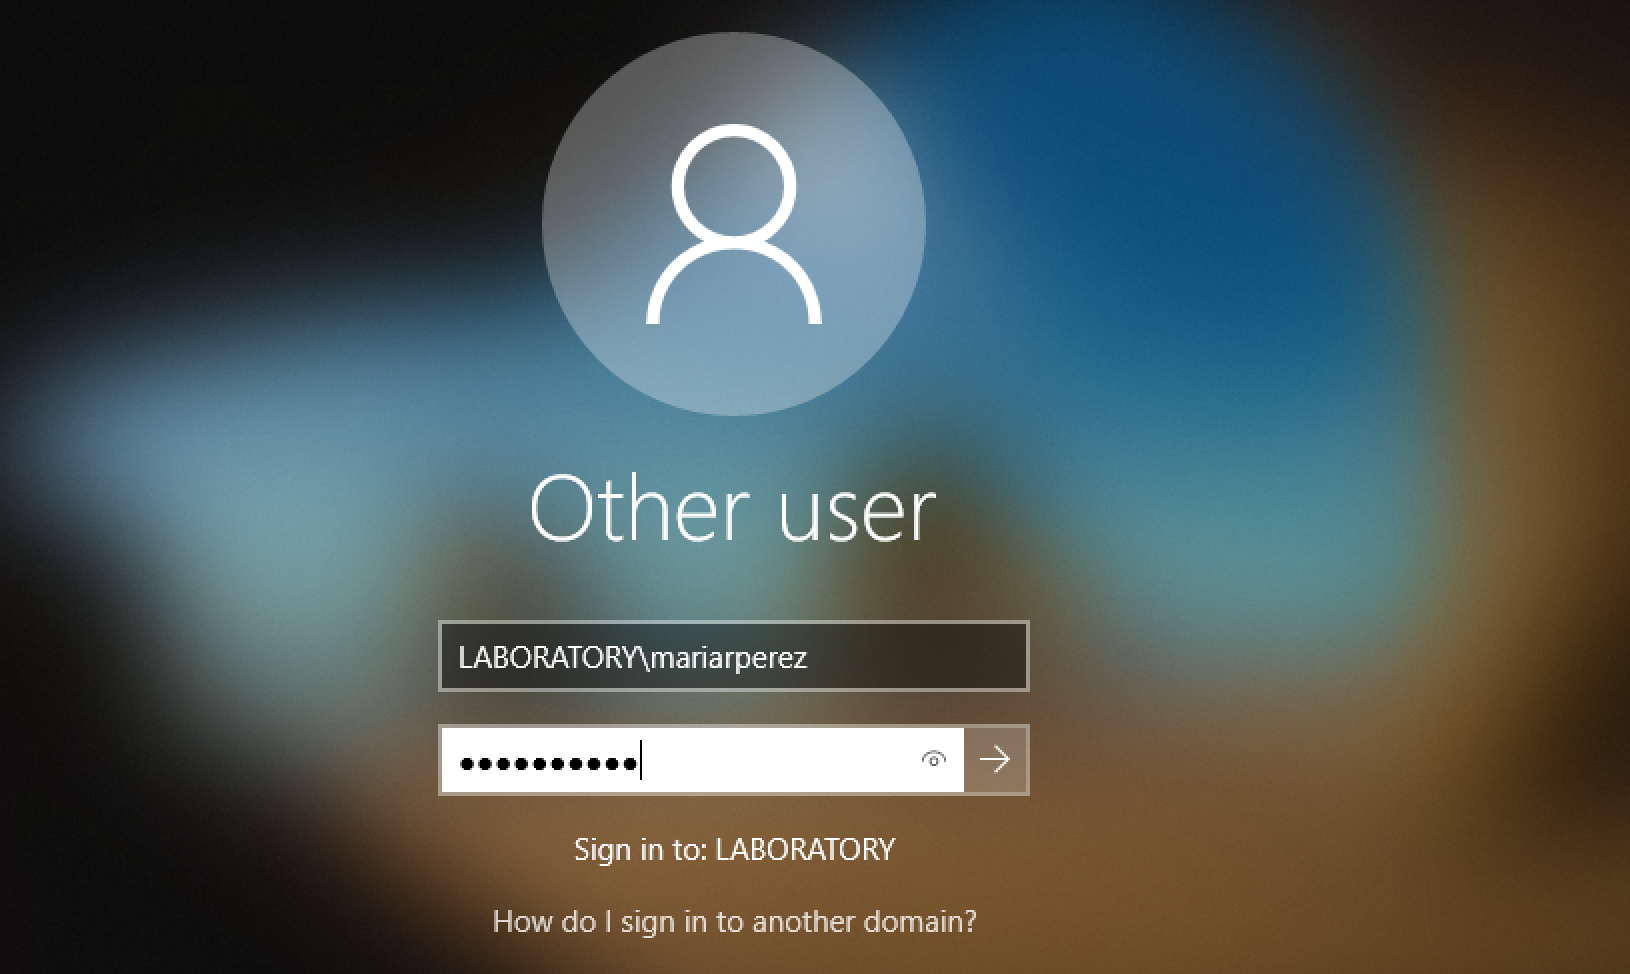
\includegraphics[width=10cm]{DC01/User6.png}
\end{center}
\caption{Inicio de sesión con la cuenta de usuario creada..}
\label{DC01-User6}
\end{figure}


\end{itemize}




\chapter{Experimentación}
En esta sección se va a detallar los principales ataques sobre Active Directory y su expemimentación en el laboratorio previamente creado. En primer lugar se va a definir en qué consiste dichos ataques y qué debilidad de los protocolos de autenticación utilizan y posteriormente se llevará a cabo una réplica de este ataque en el Active Directory {\it laboratoy.com}. \\

Para la experimentación se da por hecho que el atacante ya ha comprometido el sistema Cliente01 a través de cualquier técnica de explotación y ha conseguido escalar privilegios y dispone de una {\it Reverse Shell} interactiva. A partir de este supuesto, se realizará movimientos laterales y/o verticales a través del Active Directory. También se asume que las herramientas utilizadas están ofuscadas y eluden las protecciones de activirus que pueda tener el sistema comprometido al no presentarse en el alcance ni los objetivos de este proyecto.

\section{Pass the hash}

La idea principal del ataque {\it Pass the hash (PtH)}~\cite{Capitulo5:PtHMitre} es la autenticación de un usuario legítimo sin la necesidad de conocer la contraseña de usuario en texto claro. Para ello, el atacante únicamnete debe disponer del hash de la contraseña del usuario a suplantar. Los inicios de este ataque o técnica de movimiento lateral se retoman a 1997 cuando Paul Ashton lanzó el primer {\it Pass the hash (PtH)} con una versión de SMB modificado~\cite{Capitulo5:Paul}.\\

Como se ha observado en los capítulos previos, cuando un usuario se autentica a través del paquete de autenticación NTLM, para su autenticación el cliente cifra un secreto o nonce compartido por el servidor con el Hash NT del usuario~\cite{Capitulo5:HackingWindows}, por lo tanto, no es necesario conocer la contraseña en claro. Además, los hashes del usuario se mantiene en memoria (a través del proceso LSASS) lo que permite que, una vez autenticado un usuario legítimo, cuando el sistema requiera otra autenticación por acceder a un recurso se haga de manera trasparente al usuario.\\ 

Por lo tanto, para que llevar a cabo esta técnica, es necesario que el atacante obtenga el Hash NT del usuario al que quiera suplantar. Esta hash puede ser obtenido a través del volcado de la base de datos SAM \footnote{C:\textbackslash{}windows\textbackslash{}system32\textbackslash{}config\textbackslash{}SAM}, de copias de seguraidad o {\it backups} de esta \footnote{C:\textbackslash{}windows\textbackslash{}repair\textbackslash{}sam}, el volcado de las credenciales almacenadas por el usuario en el proceso LSASS (tiene que haber una logon sessian con dicho usuario), a través del volcado de credenciales de la base de datos NTDS  o a través de interceptar los mensajes {\it Challende-Response} cuando se autentica un usuario y crackeado el Hash NTLM para llegar a sacar el hash NT~\cite{Capitulo5:PtH}. \\

Como abstración de la capacidad de este ataque, se puede decir que {\it Pass the hash (PtH)} permite de manera efectiva la suplantación de cualquier empleado o cliente de una empresa, sin la necesidad de conocer la contraseña, únicamente conociendo el Hash NT de esta. Por lo tanto, el uso de contraseñas robustas no protegería de este tipo de ataques. \\

\subsubsection{Experimentación}

Una vez obtenido una {\it Reverse Shell} interactiva con privilegios de administrador se va a realizar la técnica de {\it Pass The Hash} a través del usuario administrador {\it federicogar}. Este usuario se ha logueado previmente en el Cliente01 por lo tanto tiene una logon session en la máquina. 

\begin{enumerate}
\item Obtenemos la {\it Reverse Shell} interactiva en la máquina atacante. Ejecutamos el comando {\it whoami} y vemos que somos el usuario de dominio {\it LABORATORY\textbackslash{}mariarperez} y no tenemos privilegios suficientes para listar el directior {\it C\$} de la máquina DC01 (Figura \ref{PTH1}).
\begin{figure}[H] %[ht!] para here [b] para bottom [t] para top
\begin{center}
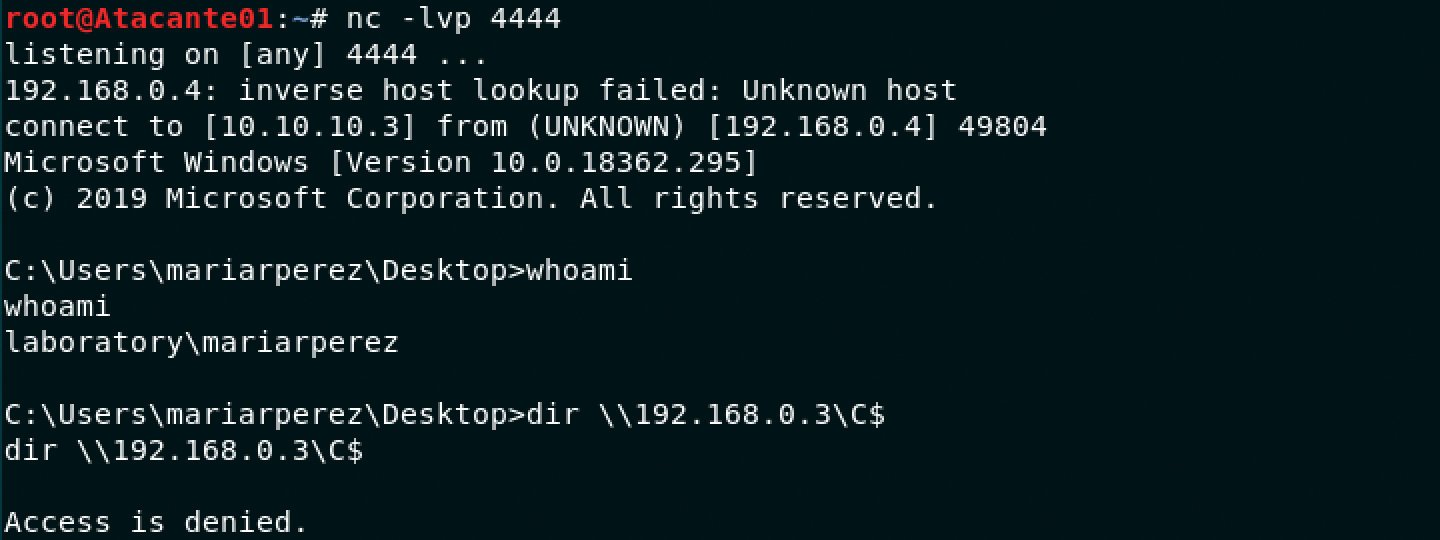
\includegraphics[width=15cm]{PTH/PTH1.png}
\end{center}
\caption{Reverse Shell interactiva sin privilegios.}
\label{PTH1}
\end{figure}

\item Si recogemos el tráfico intercambiado entre la máquina Cliente01 y el DC01, podemos ver que al intentar listar un directorio a través de la IP de éste se realiza a través del protocolo SMB utilizando el protocolo de autenticación NTLM donde el user es {\it LABORATORY\textbackslash{}mariarperez}. Al no tener privilegios, nos deniega el acceso (Figura \ref{PTH2}).
\begin{figure}[H] %[ht!] para here [b] para bottom [t] para top
\begin{center}
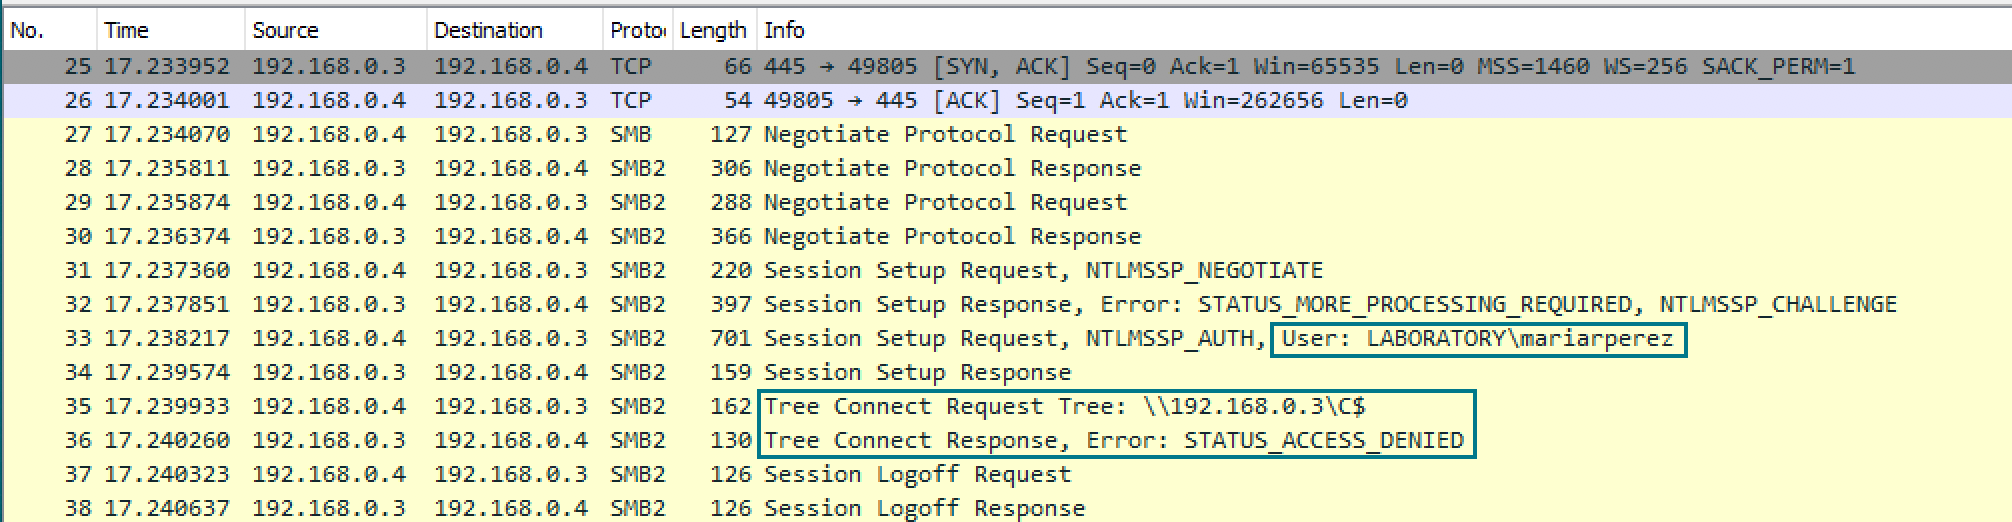
\includegraphics[width=15cm]{PTH/PTH2.png}
\end{center}
\caption{Paquetes intercambiados entre Cliente01 y DC01 - Sin pass the hash.}
\label{PTH2}
\end{figure}

\item  Al disponer de una sesión válida el usuario {\it federicogar} podemos obtener el hash de la contraseña del proceso LSASS. Para ello, se ha utilizado la herramienta Mimikatz~\cite{Capitulo5:Mimikatz} a través de los siguientes comandos (Figura \ref{PTH3}).
\begin{listing}[style=consola, numbers=none]
# privilege::debug
# sekurlsa::logonpasswords
\end{listing}

\begin{figure}[H] %[ht!] para here [b] para bottom [t] para top
\begin{center}
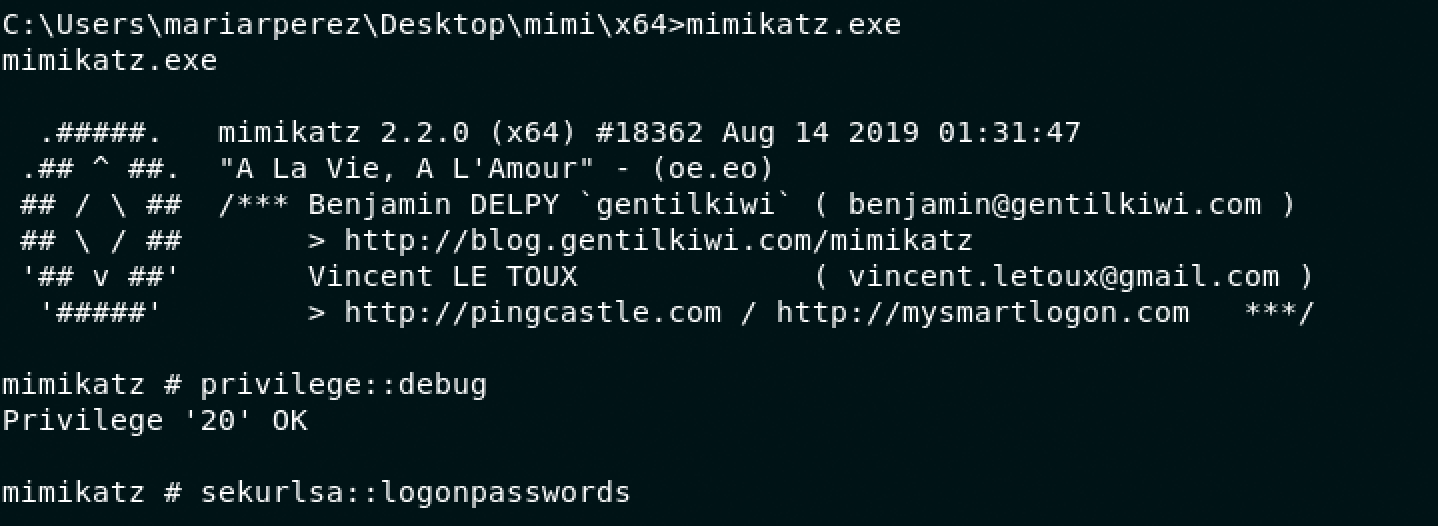
\includegraphics[width=15cm]{PTH/PTH3.png}
\end{center}
\caption{Comandos Mimikatz para listas sesiones activas.}
\label{PTH3}
\end{figure}

\item El comando anterior lista todos las sesiones activas en el usuario, por lo tanto, buscamos la que pertenece al usuario víctima y obtenmos el Hash NT (Figura \ref{PTH4}).
\begin{figure}[H] %[ht!] para here [b] para bottom [t] para top
\begin{center}
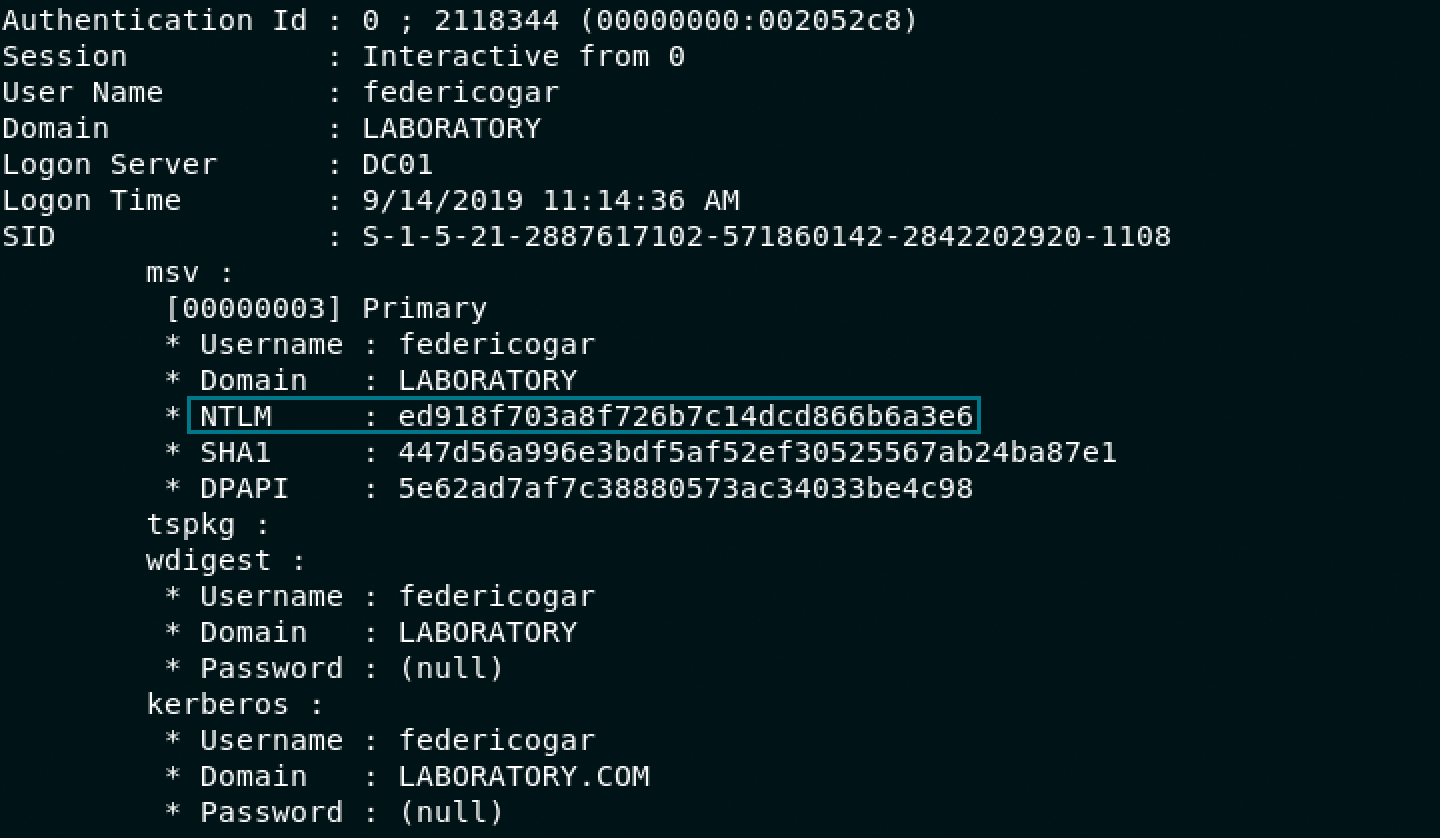
\includegraphics[width=15cm]{PTH/PTH4.png}
\end{center}
\caption{Hash del usuario víctima.}
\label{PTH4}
\end{figure}

\item La propia herramienta Mimikatz permite realizar el ataque Pass the Hash a través del siguiente comando, el resultado de este comando se puede observar en la Figura \ref{PTH5}.
\begin{listing}[style=consola, numbers=none]
# sekurlsa::pth /user:federicogar /ntlm:ed918f703a8f726b7c14dcd866b6a3e6 /domain:LABORATORY /run:cmd.exe
\end{listing}


\begin{figure}[H] %[ht!] para here [b] para bottom [t] para top
\begin{center}
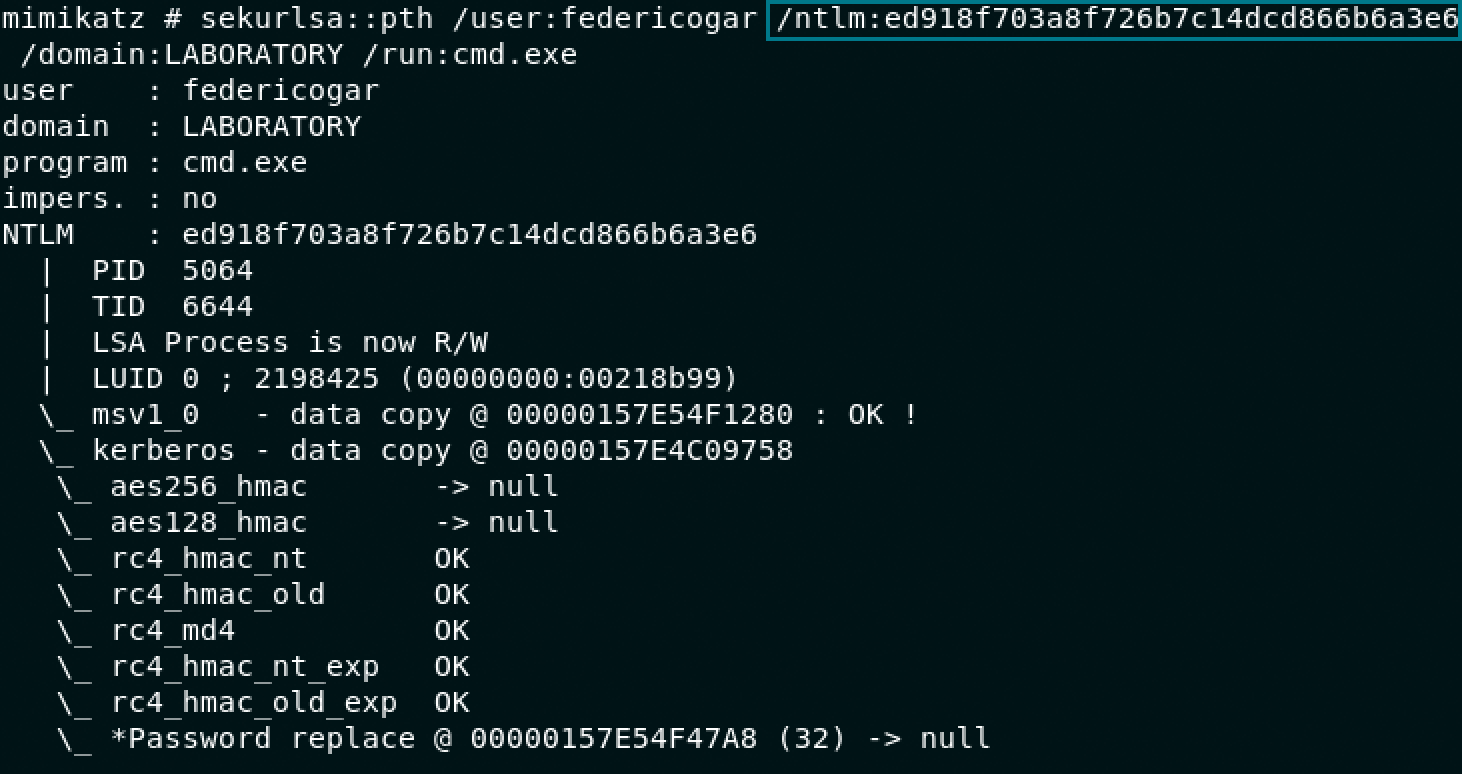
\includegraphics[width=15cm]{PTH/PTH5.png}
\end{center}
\caption{Pash the hash a través de la herramienta Mimikatz.}
\label{PTH5}
\end{figure}

\item En el comando anterior, se definió que ejecutar el comando {\it cmd.exe}, este comando se ejecutará en el Cliente01, por lo tanto, si queremos que se ejecute otra {\it Reverse Shell} con privilegios del uusario víctima sería necesario especificar otro comando. En la shell resultante (Figura \ref{PTH6}) podemos observar que aunque seguimos siendo el uusario {\it mariarperez} podemos listar los archivos de DC01. Esto es debido a que Mimikatz genera una nueva sesión para el usuario {\it mariarperez} y sobreescribe el contenido de las credenciales con el hash del otro usuario. 
\begin{figure}[H] %[ht!] para here [b] para bottom [t] para top
\begin{center}
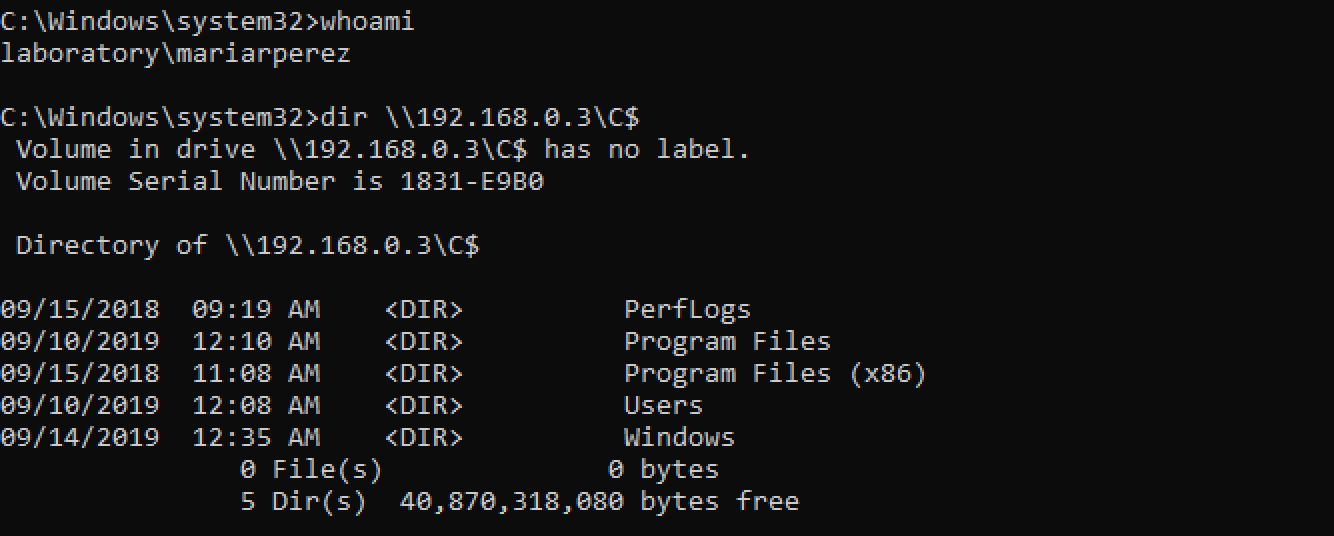
\includegraphics[width=15cm]{PTH/PTH6.png}
\end{center}
\caption{Ataque pass the hash realizado correctamente.}
\label{PTH6}
\end{figure}

\item Por último, al recoger el tráfico generado en esta comunicación podemos observar bastantes diferencias con la figura anterior, ahora el usuario es {\it federicogar} y se ha realizado el {\it Challenge-Response} de NTLM satisfactoriamente pudiendo listar los ficheros (Figura \ref{PTH7}).
\begin{figure}[H] %[ht!] para here [b] para bottom [t] para top
\begin{center}
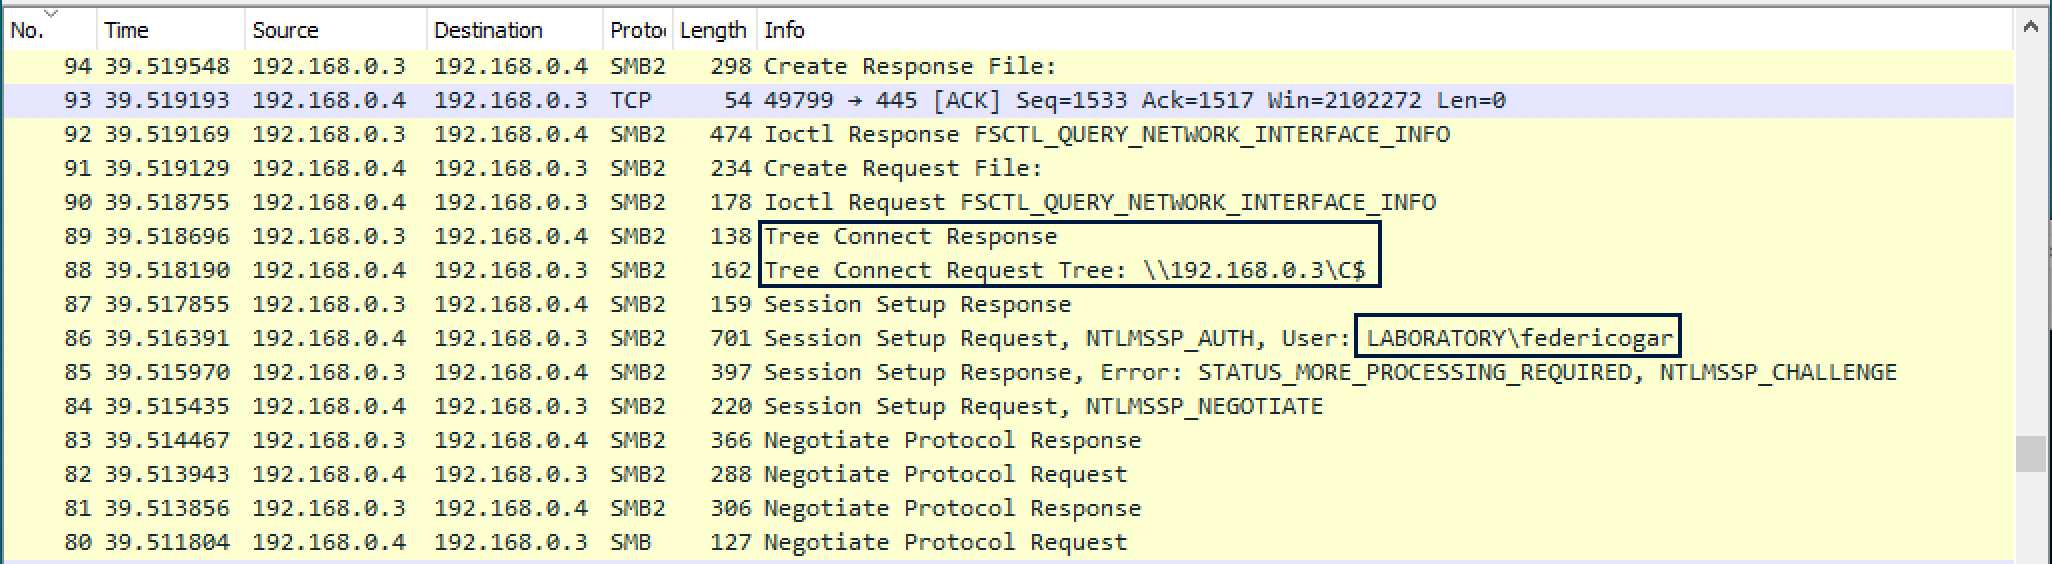
\includegraphics[width=15cm]{PTH/PTH7.png}
\end{center}
\caption{Paquetes intercambiados entre Cliente01 y DC01 - Con pass the hash.}
\label{PTH7}
\end{figure}

\end{enumerate}

\section{NTLM Relay}

Hoy en día los ataques de {\it NTLM Relay} son un técnica muy utilizada por {\it Pentesters} y atacantes permitiendo el acceso a activos o recursos crítico incluso si la organización dispone de buenas prácticas para la gestión de la seguridad. A grandes rasgos, esta técnica de movimiento lateral o vertical se puede sintetizar como un ataque de {\it pass the hash} pero a nivel de red. \\ 

Para entender este ataque es necesario entender el protocolo {\it Challenge - Respuesta} utilizado por NTLM. Aunque se ha detallado anteriormente se puede sintetizar en las siguientes fases: 

\begin{enumerate}
\item El cliente intenta iniciar sesión en un servicio o recurso.
\item El servidor responde con un desafío o {\it challenge}, es decir, el cliente dice, si eres quién dice ser, cifra este desafío con tu hash de la contraseña..
\item El cliente cifra el desafío.
\item El servidor compueba este cifrado descifradno el desafió ya que dispone del hash del usuario, si es correcto verifica al usuario. 
\end{enumerate}

En un ataque de NTLM Relay, el atacante se sitúa como intermediario entre los paquetes intercambiados en el proceso anterior. Para ello, selecciona el recurso o activo que quiere autenticarse y espera a que un usuario legítimo intente conectarse a él. A continuación se va a detallar cómo cambia el esquema de autenticación NTLM cuando se está produciendo un ataque de {\it NTLM Relay}~\cite{Capitulo5:NTLMRelay}:

\begin{enumerate}
\item En primer lugar, el cliente intenta conectarse a un recuso, esta petición es interceptada por un atacante y reenviada al servidor objetivo. 
\item El servidor contesta con un desafío, este desafío también es interceptado por el atacante y reenviado a la víctima.
\item La víctima cifra con el Hash NT de la contraseña el desafío y crea un paquete que será enviado de nuevo al atacante y este lo reenviará al servidor. 
\item El servidor comprueba que el desafío se ha cifrado correctamente y concede el acceso a dicho recurso. Por lo tanto, el atacante tiene acceso a ese recurso ya que dispone del paquete con el desafío cifrado. 
\item Por último, el atacante manda un paquete a la vítima denegando el acceso a ese recurso. 
\end{enumerate}

Como es de esperar, este tipo de ataques ha sido perseguido de cerca por Microsoft y ha implementado medidas que dificultan o imposibilitan este ataque. Una de ellas es el parche MS08-068~\cite{Capitulo5:MS08-068} que imposibilita que se puede retrasmitir un Hash NTLM a la misma máquina de la que se obtuvo imposibilitando así los ataques de NTLM Replay reflejado. Sin embargo, estos hashes se pueden retrasmitir a otros servicios o máquinas. \\

Para replicar este tipo de ataque sen el laboratorio local se va a utilizar la herramienta Responder~\cite{Capitulo5:Responder}. Antes de definir esta herramienta es necesario hablar de los {\it Windows Name Resolution}, es decir, de la forma que utilizada Microsoft para resolver los nombres de dominio. Para ello, se utilizan los protocolos: {\it Link Local Multicast Name Resolution (LLMNR)} y {\it NetBIOS over TCP/IP Name Service}. La herramienta Responder realiza un ``envenamiento'' de estos protocolos y permite obtener la credenciales en red. Esta herramienta crea servidores de autenticación como puede ser SMB, MYSQL, HTTP(s), FTP... y obliga a la víctima a enviar las credenciales a estos servidores y así poder obtenerlas. \\

Por lo tanto, con la herramienta Responder podemos obtener los Hashes NTLM de una conexión de autenticación y retrasmitirlos a través de otra herramienta como puede ser {\it ntlmrelayx.py} de la librería de Impacket o {\it MultiRelay.py}. \\

Una de las limitaciones de este ataque es que la medida que implementó Windows: SMB Signing~\cite{Capitulo5:SMBSigning} debe estar desactivado. Esta medida firma los paquetes SMB para evitar que estos sean modificados durante su retrasmisión. Se puede suponer que esta medida esta desactivada ya que en la mayoría de los Sistemas Windows están desactivadas a escepción de Windows Server como se puede ver en la Figura \ref{NTLMRelay1}.

\begin{figure}[H] %[ht!] para here [b] para bottom [t] para top
\begin{center}
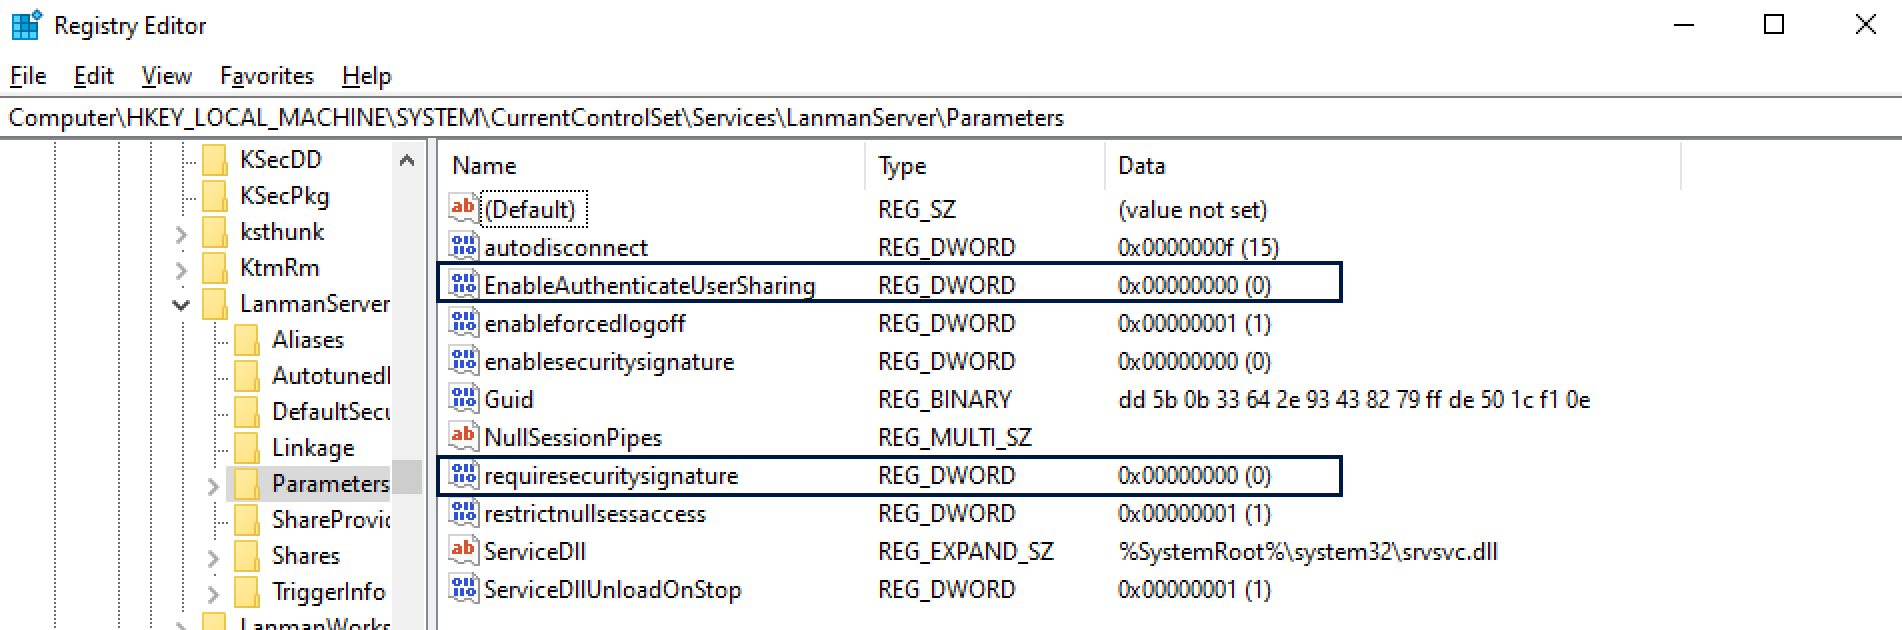
\includegraphics[width=15cm]{NTLMRelay/NTLMRelay1.png}
\end{center}
\caption{SMB Signing desactivado por defecto en Cliente01.}
\label{NTLMRelay1}
\end{figure}

\subsubsection{Experimentación}

Para ejecutar este ataque, la máquina Atacante01 tiene que estar en la misma red, para ello, desde VirtualBox añadimos una nueva tarjeta de red que esté conectada a ADNET y le asignamos la dirección IP: 192.168.0.5.

\begin{enumerate}

\item En primer lugar, descargamos la última versión de Responder de ~\cite{Capitulo5:Responder} o se utiliza la versión que trae por defecto Kali Linux, en cualquier caso se debe editar el archivo {\it Responder.conf} y deshabilitar las opciones SMB y HTTP para que estas peticiones sean recogidas por {\it ntlmrelayx.py} (Figura \ref{NTLMRelay2}
\begin{figure}[H] %[ht!] para here [b] para bottom [t] para top
\begin{center}
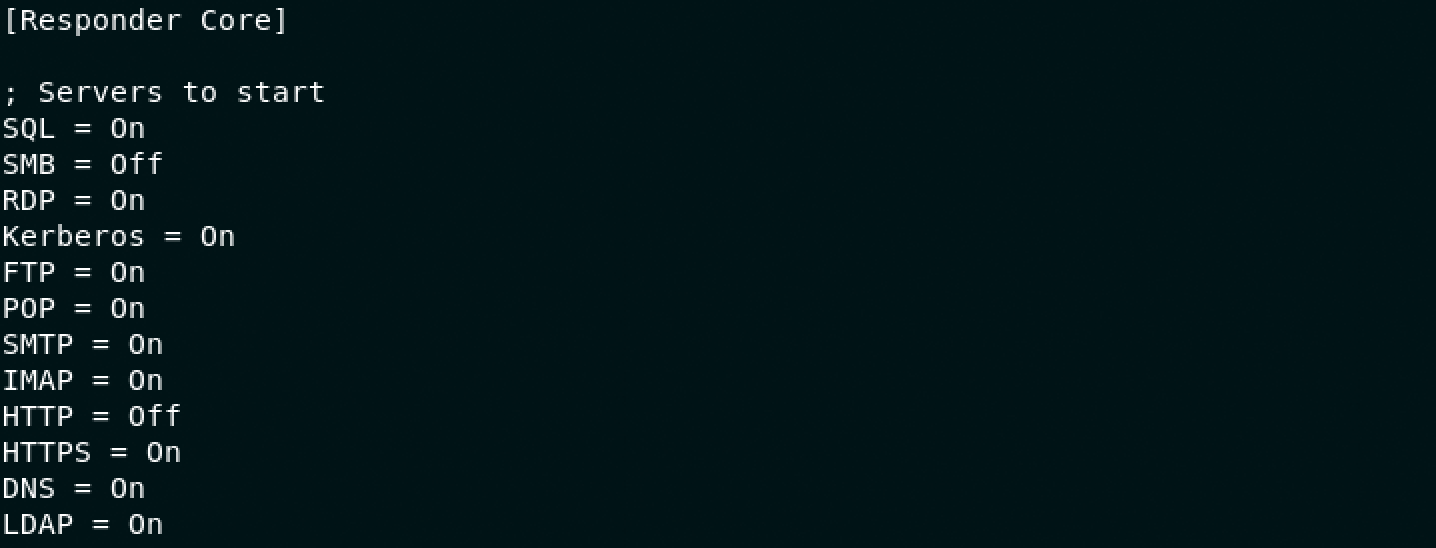
\includegraphics[width=15cm]{NTLMRelay/NTLMRelay2.png}
\end{center}
\caption{Archivo de configuración Responder.conf.}
\label{NTLMRelay2}
\end{figure}

\item Una vez editada la configuración ejecutamos el Responder. En paralelo en otra terminal ejecutamos el {\it ntlmrelayx.py} (Figura \ref{NTLMRelay3}) a través de los siguientes comandos:

\begin{listing}[style=consola, numbers=none]
# .\Responder.py -I eth2 -w -r -f -v
# ntlmrelayx.py -t 192.168.0.3 -smb2support
\end{listing}

-I eth2 - Corresponde con la interfaz de red conectada a la ADNET.
-t 192.168.0.3 - Corresponde al target, en este caso DC01. 

\begin{figure}[H] %[ht!] para here [b] para bottom [t] para top
\begin{center}
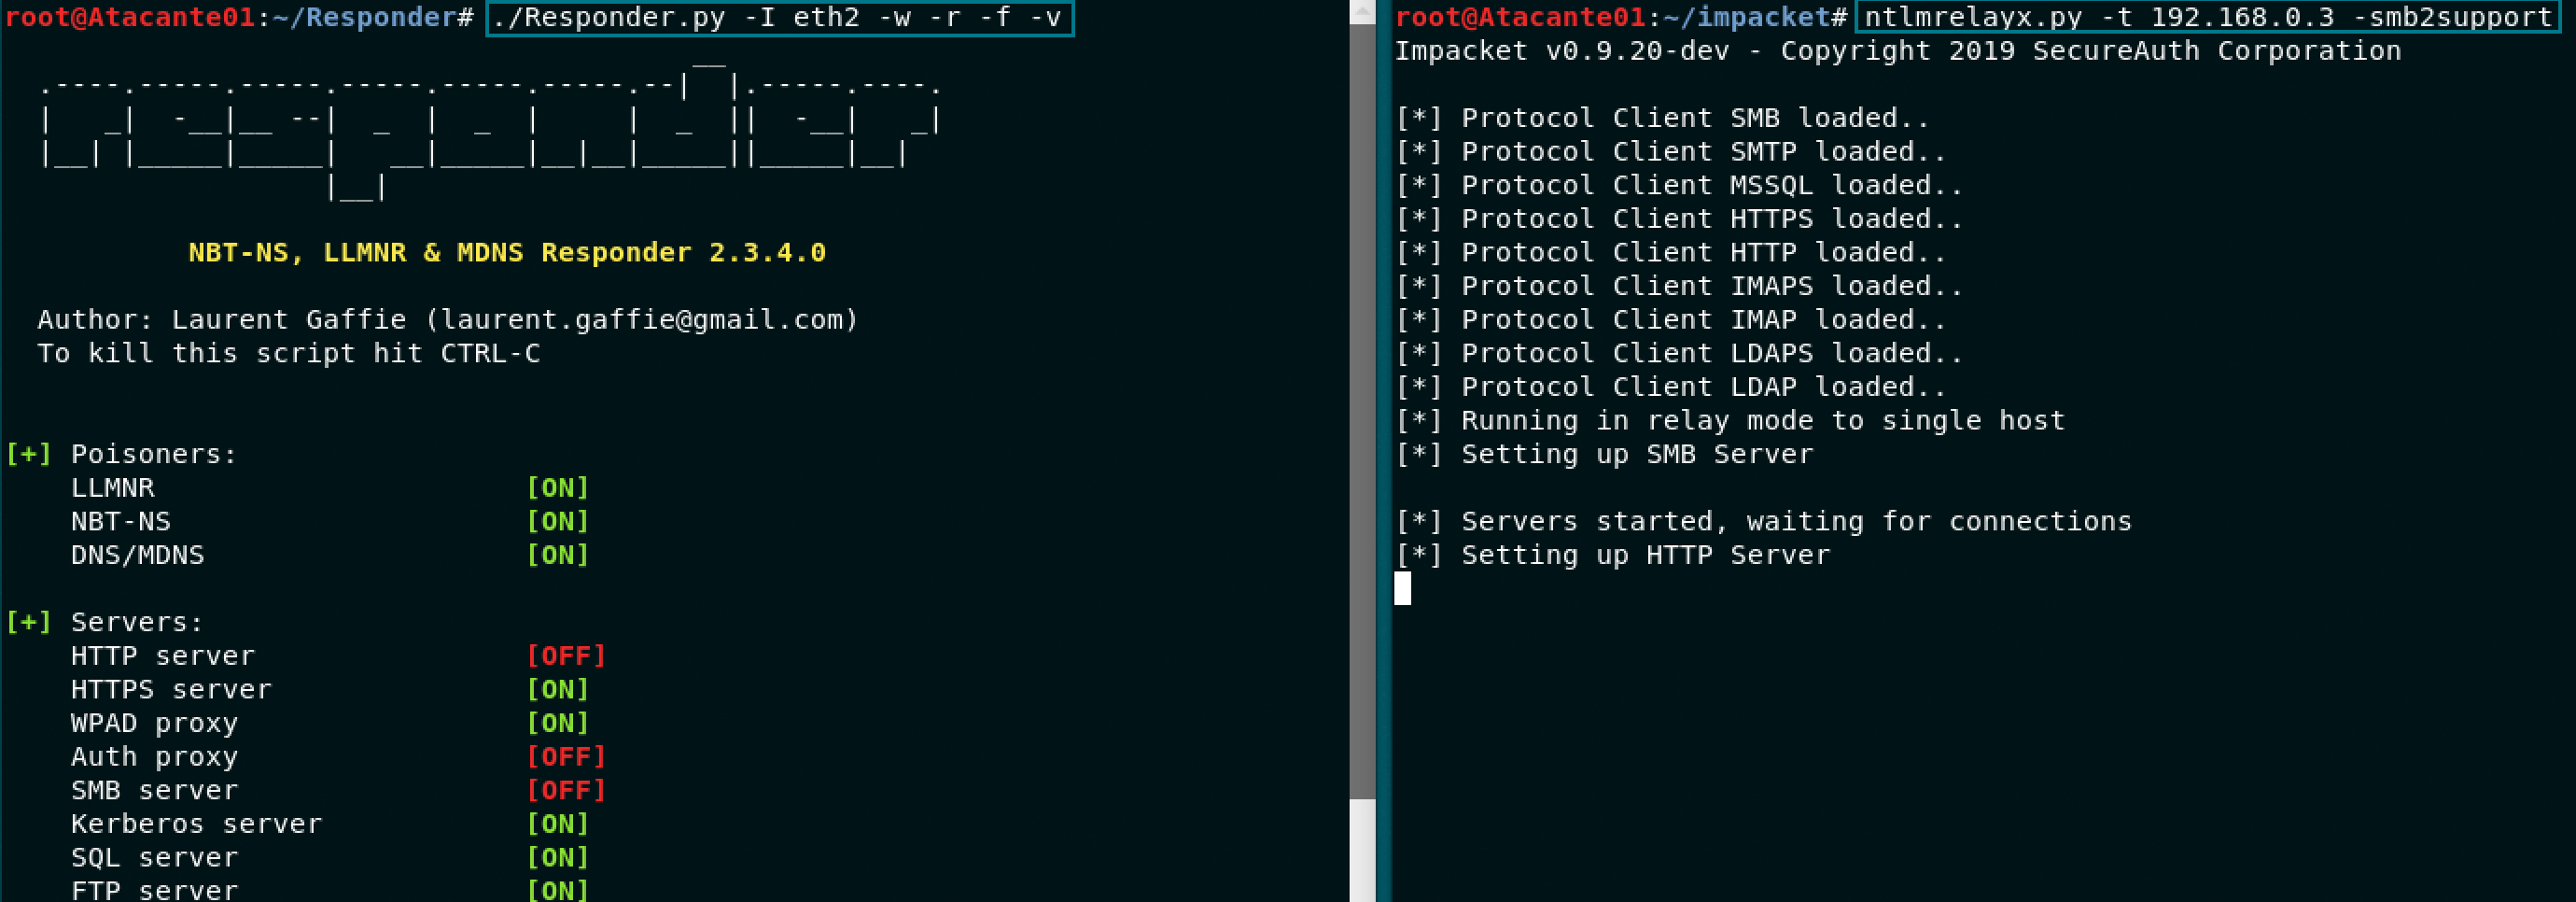
\includegraphics[width=15cm]{NTLMRelay/NTLMRelay3.png}
\end{center}
\caption{Responder y ntlmrelayx.py.}
\label{NTLMRelay3}
\end{figure}

\item Para que este ataque funcione se necesita la interacción del usuario víctima, en este caso bastaría que el usuario con privilegios de Domain Admin se conectara a un recurso inexistente como puede ser \footnote{\textbackslash{}\textbackslash{}test\textbackslash{}C\$} (Figura \ref{NTLMRelay4}).
\begin{figure}[H] %[ht!] para here [b] para bottom [t] para top
\begin{center}
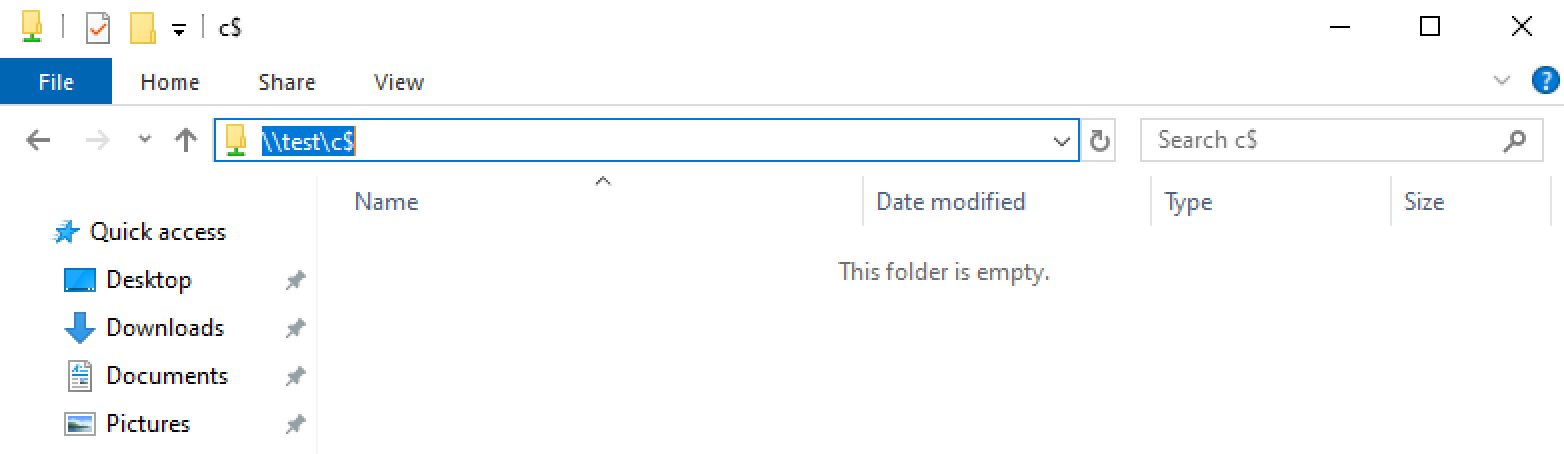
\includegraphics[width=15cm]{NTLMRelay/NTLMRelay4.png}
\end{center}
\caption{Interacción del usuario.}
\label{NTLMRelay4}
\end{figure}

\item Como se puede ver en la Figura \ref{NTLMRelay5} el ataque se ejecuta correctamente y se vuelca los datos de la SAM del Domain Controller. 
\begin{figure}[H] %[ht!] para here [b] para bottom [t] para top
\begin{center}
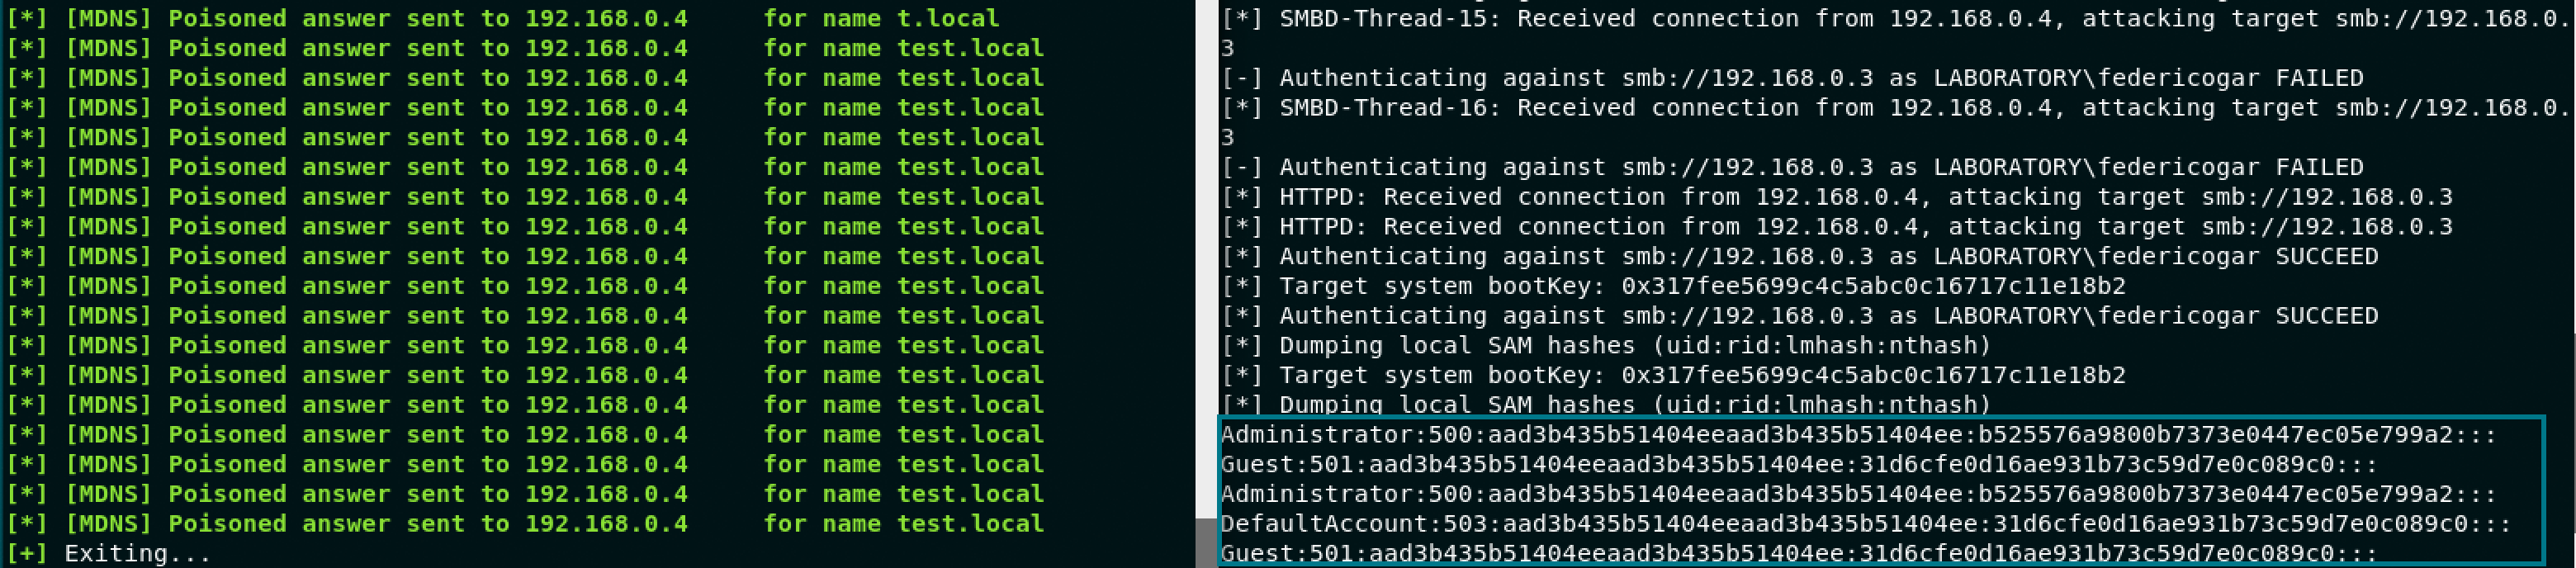
\includegraphics[width=15cm]{NTLMRelay/NTLMRelay5.png}
\end{center}
\caption{Volcado de la SAM.}
\label{NTLMRelay5}
\end{figure}

\end{enumerate}

\section{Overpass The Hash}

La técnica {\it Overpass the hash}, también conocida como {\it Pass the key (PTK)} es la equivalencia a {\it Pass the hash} para el protocolo de autenticación Kerberos. Como se ha visto anteriormente, durante el intercambio de paquetes, el usuario cifra una marca de tiempo o {\it timestamp}. En función de la versión de Kerberos se va a utilizar un secreto u otro, en este caso en las versiones más antiguas utiliza un secreto RC4 que equivale al Hash NT del usuario, en versiones más modernas utiliza claves de AES128 y AES256. Por lo tanto, con el Hash NT del usuario se puede obtener un Ticket TGT y poder realizar la autenticación correctamente.

\subsubsection{Experimentación}

\begin{enumerate}
\item En primer lugar, partimos desde una {\it Reverse Shell} interactiva con privilegios de administrador del usuario {\it mariarperez} y tratamos de listar el directorio {\it C\$} del DC01 a través de protocolo de Kerberos(Figura \ref{OTH1}).
\begin{figure}[H] %[ht!] para here [b] para bottom [t] para top
\begin{center}
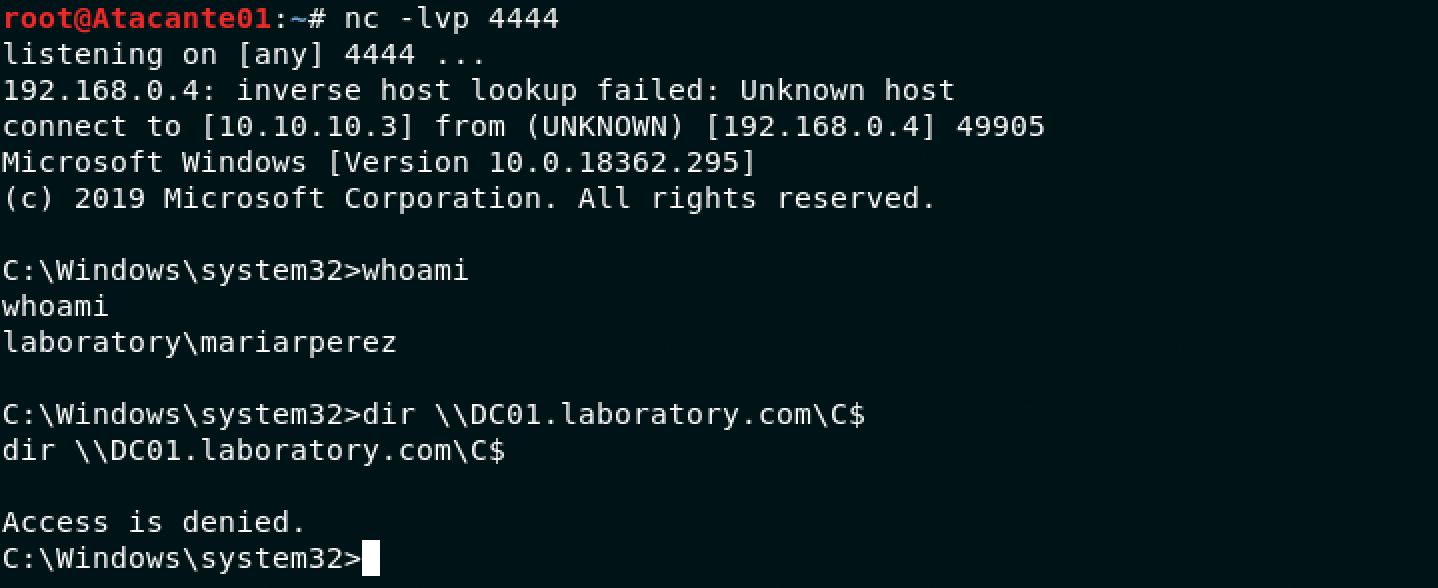
\includegraphics[width=15cm]{OTH/OTH1.png}
\end{center}
\caption{Reverse Shell interactiva.}
\label{OTH1}
\end{figure}

\item Como se puede ver en Wireshark, el intercambio de paquetes KRB5 falla (Figura \ref{OTH2}).
\begin{figure}[H] %[ht!] para here [b] para bottom [t] para top
\begin{center}
\includegraphics[width=15cm]{OTH/OTH2.png}
\end{center}
\caption{Intercambio de paquetes de Kerberos.}
\label{OTH2}
\end{figure}

\item Repetimos los pasos hechos en {\it Pass the hash}, listamos las sesiones activas y obtenemos el hash de la contraseña MD5 (Figura \ref{OTH3} y Figura \ref{OTH4}).
\begin{figure}[H] %[ht!] para here [b] para bottom [t] para top
\begin{center}
\includegraphics[width=15cm]{OTH/OTH3.png}
\end{center}
\caption{Comandos Mimikatz para listas sesiones activas.}
\label{OTH3}
\end{figure}

\begin{figure}[H] %[ht!] para here [b] para bottom [t] para top
\begin{center}
\includegraphics[width=15cm]{OTH/OTH4.png}
\end{center}
\caption{Hash del usuario víctima.}
\label{OTH4}
\end{figure}

\item Realizamos el ataque a través del mismo comando que en {\it Pass the hash} (Figura \ref{OTH5}).
\begin{figure}[H] %[ht!] para here [b] para bottom [t] para top
\begin{center}
\includegraphics[width=15cm]{OTH/OTH5.png}
\end{center}
\caption{Pash the hash a través de la herramienta Mimikatz.}
\label{OTH5}
\end{figure}

\item Se ejecuta el comando especificado en el comando anterior, en este caso un {\it cmd.exe} en el que podemos acceder al directorio (Figura \ref{OTH6}).
\begin{figure}[H] %[ht!] para here [b] para bottom [t] para top
\begin{center}
\includegraphics[width=15cm]{OTH/OTH6.png}
\end{center}
\caption{Ataque over-pass the hash realizado correctamente..}
\label{OTH6}
\end{figure}

\item En los paquetes KRB5 intercambiados podemos ver que se usa RC4 (Figura \ref{OTH7}) y que la autenticación se completa correctamente recibiendo así un Ticket TGT. 
\begin{figure}[H] %[ht!] para here [b] para bottom [t] para top
\begin{center}
\includegraphics[width=15cm]{OTH/OTH7.png}
\end{center}
\caption{Intercambio de paquetes de Kerberos.}
\label{OTH7}
\end{figure}


\end{enumerate}




\section{Pass The Ticket}

\section{Golden/Silver Ticket}

asection{Kerberoast}


\chapter{Resultados}
En este capítulo se van a discutir los resultados obtenidos tanto en la creación del laboratorio como la experimetnación de los principales ataques que afectan a Active Directory en la última versión de Windows Server 2019.

\subsubsection{Creación del laboratorio}
El laboratorio propuesto para la implentación de las pruebas realizadas consta de 4 máquinas: en primer lugar DC01 representa el Domain Controller que gestiona Active Directory formada por un Windows Server 2019, en segundo lugar la máquina Cliente01 representa a un usuario o empleado (o varios usuarios) unidos al dominio cuya máquina puede ser comprometida, en tercer lugar la máquina Gateway que sirve de enlace entre la red interna y la red externa que representa internet, por último, la máquina denominada Atacante01 representa un atacante, miembro de Red Team o auditor de seguridad que compromete un sistema del dominio y tiene acceso a la red interna. Se ha comprobado que con estas cuatro máquinas es posible replicar los ataques planteados en el Capítulo de experimentación. 
\subsubsection{Pass the hash}
En cuanto al ataque de Pass The Hash, se ha comprobado que es posible replicarlo en entornos actualizados, la premisa para este ataque es comprometer un sistema de dominio con suficientes privilegios como para obtener las credenciales almacenadas en el equipo de un cliente. El enfoque más efectivo para la protección de un equipo frente a este tipo de ataques es implementar políticas de seguridad para que hashes de cuentas privilegiadas como puede ser de {\it Domain Admin} no se almacenen en memoria o sea imposible extraer dichos hashes.
\subsubsection{NTLM Relay}
Para evitar ataques de NTLM Relay, Microsoft ha implementado varias medidas, entre ellas y la más efectiva ha sido incluida en el parche MS08-068 que imposibilita ataques de NTLM Reflejado, es decir, que no es posible transmitir el Hash NTLM a la misma máquina que se obtuvo, aunque como se ha visto en la literatura es posible enviarlo a otro servicio o recurso. Por otro lado, la otra medida es la firma de los paquetes SMB para evitar que el mensaje se altere y proteger la integridad del mensaje. Esta medida imposibilita los ataques de SMB Relay basados en el protocolo SMB aunque esta medida no está activada por defecto en la mayoría de los equipos con sistema operativo Windows. Pese a estas medidas, se ha comprobado la eficacia de este ataque ya que la única premisa es que el atacante esté en la misma red que el dominio y ha sido posible realizar un volcado de la base de datos SAM. 
\subsubsection{Overpass the hash}
Este ataque ha sido posible realizarlo del mismo modo que el ataque {\it pass the hash}. {\it Overpass the hash} permite realizar estos ataques en el paquete de autenticación Kerberos, ampliamente utilizado para la autenticación en servicios y recursos utilizados por Active Directory.
\subsubsection{Pass the ticket}
La eficacia del ataque {\it pass the ticket} reside en la obtención de un Ticket TGT válido que resulte de interés para acceder a recursos importantes como puede ser un Domain Controller o equipos con información confidencial. A diferencia de ataques de {\it pass the hash u overpass the hash} no es necesario tener una sesión de administrador local para obtener los Tickets TGS algo que puede ser de utilidad cuando no se ha conseguido elevar privilegios en una máquina comprometida.
\subsubsection{Golden Ticket}
La técnica {\it Golden Ticket} te permite mantener persistencia una vez comprometido un Domain Controller de manera eficaz y transparente a los administradores de sistemas. Es necesario disponer del hash de la contraseña de administración {\it krbtgt} lo dificulta la realización de este ataque. Una vez obtenida, se ha comprobado que es posible obtener tickets TGT suplantando a cualquier usuario del dominio algo que puede ser crítico para organizaciones y empresas. 
\subsubsection{Kerberoast}
Por último, el ataque Kerberoast es el menos ``ruidoso'' ya que únicamente se realizan peticiones legítimas al dominio y una vez obtenidos los tickets TGS se puede realizar la fase de cracking en una máquina local ajena al dominio. Pese a ello, este ataque reside su eficacia en credenciales débiles de los servicios y recursos lo que dificulta así su efectividad. 


\chapter{Conclusiones y trabajo futuro}

\section{Conclusiones}

A lo largo del trabajo se han revisado en profundidad las diferentes técnicas y ataques que puedes comprometer la seguridad de un Active Directory en la última versión proporcionada por Micorosft: Windows Server 2019. Se ha implementado un laboratorio local que permite la replicación de dichos ataques y diferentes pruebas en un entorno controlado sin afectar a una implementación de una empresa u organización. Esto ha requerido la instalción de difernetes sistemas operativos, la configuración de una topología de red que puede simular a un entorno real, la configuración de Active Directory y la creación de diferentes usuarios con distintos privilegios. Una vez montado el laboratorio de pruebas ha sido posible replicar dichos ataques de manera satisfactoria. \\

En cuanto a la experimentación realizada, todos los ataques elegidos se han podido replicar de manera satisfactoria en la última versión de Windows Server, por lo que se puede concluir que, aún siguiendo una política de actualizaciones es posible que se pueda comprometer un servicio de directorio como Active Directory de una empresa. En las últimas actualizaciones, Microsoft, ha intentado mitigar estos ataques o al menos reducir su impacto implemtando medidas como las vistas anteriormente. En técnicas como Pass the hash, es posible que no sea una vulnerabilidad como tal sino una implmentación al modelo de {\it Singl Sign-On (SSO)} que permite al usuario acceder a recursos y servicios sin introducir la contraseña cada vez que se requiera autenticación. \\

La realización de este proyecto ha servido para adquirir una base en Active Directory y conocer los principales ataques utilizados por atacantes y profesionales de la seguridad informática. El conocimiento adquirido es de gran importancia hoy en día debido a la multitud de empresas que utilizan Active Directory como servicio de directorio para gestionar los recursos en red.\\

\section{Trabajo Futuro}

A lo largo de este proyecto se han encontrado limitaciones que han sido asumidas y definidas fuera del alcance de este proyecto, como puede ser la fase de enumeración, acceso inicial, explotación y elevación de privilegios en Sistemas Windows centrando este proyecto en movimientos laterales y movimientos verticales a través de una red. Por lo que se define como objeto de estudio futuro las fases previas a la compromisión de un sistema. \\

En cuanto al laboratorio, este trabajo se ha centrado en un único dominio {\it Laboratory.com} como objeto de estudio. Las empresas de hoy en día disponen de multitud de forest, dominios y subdominios debido a la gran cantidad de recurosso a gestionar, por lo que sería interesante ampliar el laboratorio con distintos forest y dominios y envestigar cómo gestiona Windows las relaciones de confianza entre ellos. \\

Por último, en cuanto a los ataque sería de gran utilidad probar diferentes variaciones a dichos ataques o la experimentación de otros ataques interesantes como {\it DCSync}. Otra de las limitaciones asumidas a lo largo del desarrollo del trabajo ha sido la utilización de herramientas como Mimikatz. Estas herramientas son objeto de estudio por los antivirus y es importante que el ataque no sea detectado por administradores de sistemas o el equipo de {\it Blue Team}. Por lo tanto, como trabaja futuro sería la investigación de dichas herramientas y la detección que hacen activirus como Windows Defender.



%----------
%	BIBLIOGRAFÍA
%----------	

%\nocite{*} % Si quieres que aparezcan en la bibliografía todos los documentos que la componen (también los que no estén citados en el texto) descomenta está lína

\clearpage
\addcontentsline{toc}{chapter}{Bibliografía}
%\setquotestyle[english]{british} % Cambiamos el tipo de cita porque en el estilo IEEE se usan las comillas inglesas.
%\printbibliography

\bibliography{Bibliografia/Bibliografia}{}
\bibliographystyle{ieeetr}


%----------
%	ANEXOS
%----------	

% Si tu trabajo incluye anexos, puedes descomentar las siguientes líneas
% \chapter*{Instalación Windows Server 2019 (DC01)}
%\pagenumbering{gobble} % Las páginas de los anexos no se numeran
%\addcontentsline{toc}{chapter}{Anexo 1: Instalación Windows Server 2019 (DC01)}
%\textbf{Creación de Máquina Virtual}
\begin{enumerate}
\item Test.
\begin{figure}[H] %[H] para here [b] para bottom [t] para top
\begin{center}
\includegraphics[width=10cm]{DC01/MV1.png}
\end{center}
\end{figure}

\item Test
\begin{figure}[H] %[H] para here [b] para bottom [t] para top
\begin{center}
\includegraphics[width=10cm]{DC01/MV2.png}
\end{center}
\end{figure}

\item Test
\begin{figure}[H] %[H] para here [b] para bottom [t] para top
\begin{center}
\includegraphics[width=10cm]{DC01/MV3.png}
\end{center}
\end{figure}

\item Test
\begin{figure}[H] %[H] para here [b] para bottom [t] para top
\begin{center}
\includegraphics[width=10cm]{DC01/MV4.png}
\end{center}
\end{figure}

\item Test
\begin{figure}[H] %[H] para here [b] para bottom [t] para top
\begin{center}
\includegraphics[width=10cm]{DC01/MV5.png}
\end{center}
\end{figure}

\item Test
\begin{figure}[H] %[H] para here [b] para bottom [t] para top
\begin{center}
\includegraphics[width=10cm]{DC01/MV6.png}
\end{center}
\end{figure}

\item Test
\begin{figure}[H] %[H] para here [b] para bottom [t] para top
\begin{center}
\includegraphics[width=10cm]{DC01/MV7.png}
\end{center}
\end{figure}

\end{enumerate}



\textbf{Instalación}

\begin{enumerate}
\item Una vez creada la máquina virtual se ejecuta la instacia y se procede a la instalación.
\item En primer lugar, se elige el idioma y el teclado a utilizar. En este caso se ha utilizado la imagen (iso) de Windows Server 2019 en inglés: English (United States) y el teclado en español: Spanish (Spain, International Sort) y spanish como método de entrada.

\begin{figure}[H] %[H] para here [b] para bottom [t] para top
\begin{center}
\includegraphics[width=10cm]{DC01/Instalacion1.png}
\end{center}
\end{figure}

\item Se empieza con la instalación pulsando en ``Install Now''.

\begin{figure}[H] %[H] para here [b] para bottom [t] para top
\begin{center}
\includegraphics[width=10cm]{DC01/Instalacion2.png}
\end{center}
\end{figure}


\item Test

\begin{figure}[H] %[H] para here [b] para bottom [t] para top
\begin{center}
\includegraphics[width=10cm]{DC01/Instalacion3.png}
\end{center}
\end{figure}

\item Test

\begin{figure}[H] %[H] para here [b] para bottom [t] para top
\begin{center}
\includegraphics[width=10cm]{DC01/Instalacion4.png}
\end{center}
\end{figure}

\item Test

\begin{figure}[H] %[H] para here [b] para bottom [t] para top
\begin{center}
\includegraphics[width=10cm]{DC01/Instalacion5.png}
\end{center}
\end{figure}

\item Test

\begin{figure}[H] %[H] para here [b] para bottom [t] para top
\begin{center}
\includegraphics[width=10cm]{DC01/Instalacion6.png}
\end{center}
\end{figure}

\item Test

\begin{figure}[H] %[H] para here [b] para bottom [t] para top
\begin{center}
\includegraphics[width=10cm]{DC01/Instalacion7.png}
\end{center}
\end{figure}

\item Test

\begin{figure}[H] %[H] para here [b] para bottom [t] para top
\begin{center}
\includegraphics[width=10cm]{DC01/Instalacion8.png}
\end{center}
\end{figure}

\end{enumerate}


\textbf{Actualización}

\begin{enumerate}
\item Test

\begin{figure}[H] %[H] para here [b] para bottom [t] para top
\begin{center}
\includegraphics[width=10cm]{DC01/Update1.png}
\end{center}
\end{figure}

\item Test

\begin{figure}[H] %[H] para here [b] para bottom [t] para top
\begin{center}
\includegraphics[width=10cm]{DC01/Update2.png}
\end{center}
\end{figure}

\end{enumerate}

\textbf{Configuración}



%
%\chapter*{Instalación Windows 10 Enterprise (Cliente01)}
%\addcontentsline{toc}{chapter}{Anexo 2: Instalación Windows 10 Enterprise (Cliente01)}
%\textbf{Creación de Máquina Virtual}
\begin{enumerate}

\item En primer lugar, elegimos el nombre de la máquina: \textbf{Cliente01} y el tipo, en este caso se trata de \textbf{Microsoft Windows} versión \textbf{Microsoft Windows 10 (64-bit)}.
\begin{figure}[H] %[H] para here [b] para bottom [t] para top
\begin{center}
\includegraphics[width=10cm]{Cliente01/MV1.png}
\end{center}
\end{figure}

\item En el segundo paso, elegimos la RAM que vamos a destinar a la máquina virtual, aunque el requisito mínimo es de 2GB vamos a destinar 4GB: \textbf{4096 MB} para mejorar la experiencia a la hora de usar esta máquina.
\begin{figure}[H] %[H] para here [b] para bottom [t] para top
\begin{center}
\includegraphics[width=10cm]{Cliente01/MV2.png}
\end{center}
\end{figure}

\item En esta opción, se elige \textbf{Crear un disco duro virtual ahora}.
\begin{figure}[H] %[H] para here [b] para bottom [t] para top
\begin{center}
\includegraphics[width=10cm]{Cliente01/MV3.png}
\end{center}
\end{figure}

\item En cuanto al tipo de disco duro virtual se elige \textbf{VDI (Virtualbox Disk Image)}.
\begin{figure}[H] %[H] para here [b] para bottom [t] para top
\begin{center}
\includegraphics[width=10cm]{Cliente01/MV4.png}
\end{center}
\end{figure}

\item Por último, se ha elegido \textbf{30 GBs} de espacio de disco duro virtual.
\begin{figure}[H] %[H] para here [b] para bottom [t] para top
\begin{center}
\includegraphics[width=10cm]{Cliente01/MV5.png}
\end{center}
\end{figure}

\item Para arrancar la imagen del sistema operativo, hay que seleccionarla desde Con\-fi\-gu\-ra\-ción/\-Almacenamiento de la máquina virtual creada como Unidad Óptica.
\begin{figure}[H] %[H] para here [b] para bottom [t] para top
\begin{center}
\includegraphics[width=10cm]{Cliente01/MV6.png}
\end{center}
\end{figure}




\end{enumerate}
\textbf{Instalación}

\textbf{Actualización}

%
%
%\chapter*{Instalación Debian 10 (Gateway)}
%\addcontentsline{toc}{chapter}{Anexo 3: Instalación Debian 10 (Gateway)}
%\textbf{Creación de Máquina Virtual}
\begin{enumerate}

\item En primer lugar, elegimos el nombre de la máquina: \textbf{Gateway} y el tipo, en este caso se trata de \textbf{Linux} versión \textbf{Debian (64-bit)}.
\begin{figure}[H] %[H] para here [b] para bottom [t] para top
\begin{center}
\includegraphics[width=10cm]{Gateway/MV1.png}
\end{center}
\end{figure}

\item En el segundo paso, elegimos la RAM que vamos a destinar a la máquina virtual, al tratarse de un Debian sin entorno gráfico no es necesario destinarle muchos requisos por lo que elegimos 1GB: \textbf{1024 MB}.
\begin{figure}[H] %[H] para here [b] para bottom [t] para top
\begin{center}
\includegraphics[width=10cm]{Gateway/MV2.png}
\end{center}
\end{figure}

\item En esta opción, se elige \textbf{Crear un disco duro virtual ahora}.
\begin{figure}[H] %[H] para here [b] para bottom [t] para top
\begin{center}
\includegraphics[width=10cm]{Gateway/MV3.png}
\end{center}
\end{figure}

\item En cuanto al tipo de disco duro virtual se elige \textbf{VDI (Virtualbox Disk Image)}.
\begin{figure}[H] %[H] para here [b] para bottom [t] para top
\begin{center}
\includegraphics[width=10cm]{Gateway/MV4.png}
\end{center}
\end{figure}

\item Por último, se ha elegido \textbf{10 GBs} de espacio de disco duro virtual.
\begin{figure}[H] %[H] para here [b] para bottom [t] para top
\begin{center}
\includegraphics[width=10cm]{Gateway/MV5.png}
\end{center}
\end{figure}

\item Para arrancar la imagen del sistema operativo, hay que seleccionarla desde Con\-fi\-gu\-ra\-ción/\-Almacenamiento de la máquina virtual creada como Unidad Óptica.
\begin{figure}[H] %[H] para here [b] para bottom [t] para top
\begin{center}
\includegraphics[width=10cm]{Gateway/MV6.png}
\end{center}
\end{figure}




\end{enumerate}
\textbf{Instalación}

\textbf{Actualización}

%
%
%\chapter*{Instalación Kali Linux 2019.3 (Atacante01)}
%\addcontentsline{toc}{chapter}{Anexo 4: Instalación Kali Linux 2019.3 (Atacante01)}
%\textbf{Creación de Máquina Virtual}
\begin{enumerate}

\item En primer lugar, elegimos el nombre de la máquina: \textbf{Atacante01} y el tipo, en este caso se trata de \textbf{Linux} versión Kali Linux 2019.3, como esta opción no está disponible elegimos \textbf{Other Linux (64-bit)}.
\begin{figure}[H] %[H] para here [b] para bottom [t] para top
\begin{center}
\includegraphics[width=10cm]{Atacante01/MV1.png}
\end{center}
\end{figure}

\item En el segundo paso, elegimos la RAM que vamos a destinar a la máquina virtual, al tratarse de la máquina donde se van a realizar las pruebas se destinan 4GB: \textbf{4096 MB}.
\begin{figure}[H] %[H] para here [b] para bottom [t] para top
\begin{center}
\includegraphics[width=10cm]{Atacante01/MV2.png}
\end{center}
\end{figure}

\item En esta opción, se elige \textbf{Crear un disco duro virtual ahora}.
\begin{figure}[H] %[H] para here [b] para bottom [t] para top
\begin{center}
\includegraphics[width=10cm]{Atacante01/MV3.png}
\end{center}
\end{figure}

\item En cuanto al tipo de disco duro virtual se elige \textbf{VDI (Virtualbox Disk Image)}.
\begin{figure}[H] %[H] para here [b] para bottom [t] para top
\begin{center}
\includegraphics[width=10cm]{Atacante01/MV4.png}
\end{center}
\end{figure}

\item Por último, se ha elegido \textbf{15 GBs} de espacio de disco duro virtual.
\begin{figure}[H] %[H] para here [b] para bottom [t] para top
\begin{center}
\includegraphics[width=10cm]{Atacante01/MV5.png}
\end{center}
\end{figure}

\item Para arrancar la imagen del sistema operativo, hay que seleccionarla desde Con\-fi\-gu\-ra\-ción/\-Almacenamiento de la máquina virtual creada como Unidad Óptica.
\begin{figure}[H] %[H] para here [b] para bottom [t] para top
\begin{center}
\includegraphics[width=10cm]{Atacante01/MV6.png}
\end{center}
\end{figure}




\end{enumerate}
\textbf{Instalación}

\textbf{Actualización}




\end{document}
